\section{Linear Prediction}
Linear Prediction (LP) is proposed in order to compensate for the delay introduced by sampling and reconstructing acoustical signals. The delays have high impact on the performance of an ANC system. \\
The proposed predictor uses Wiener filtering to predict the next sample based on the autocorrelation (ACF) of some previous samples. The prediction algorithm is then coupled in cascade in order to predict multiple samples. 

\begin{figure}[H]
	\centering
	\tikzsetnextfilename{WienerHopf}
	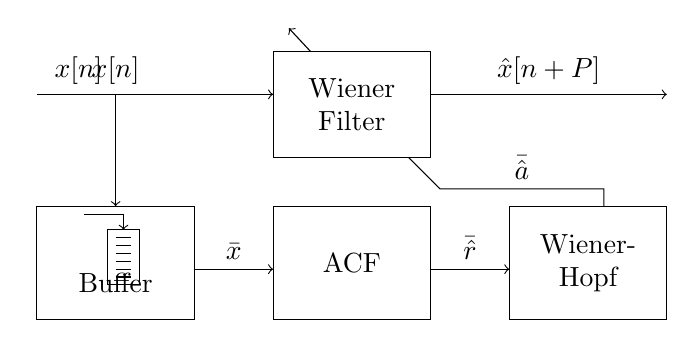
\begin{tikzpicture}

%% Boxes
\draw  (-3,3) rectangle node[text width=2cm,align=center] {Wiener Filter}(-1,4.34);
\draw  (-1,2.38) rectangle node[text width=2cm,align=center] {ACF}(-3,0.94);
\draw  (-4,2.38) rectangle node[text width=2cm,align=center,below=.25] {Buffer}(-6,0.94);
\draw  (0,2.38) rectangle node[text width=1.5cm,align=center] {Wiener- Hopf}(2,0.94);



%%Buffer
\draw (-4.7,1.38) node (v1) {} -- (-5.1,1.38) -- (-5.1,2.08) -- (-4.7,2.08) -- (-4.7,1.38);
\draw (-5,1.98) -- (-4.8,1.98);
\draw (-5,1.88) -- (-4.8,1.88);
\draw (-5,1.78) -- (-4.8,1.78);
\draw (-5,1.68) -- (-4.8,1.68);
\draw (-5,1.58) -- (-4.8,1.58);
\draw (-5,1.48) -- (-4.8,1.48);
\draw [->](-5.4,2.28) -- (-4.9,2.28) -- (-4.9,2.08);


%% Lines
\draw [->](-4,1.58) -- node[above]{$\bar{x}$} (-3,1.58);
\draw [->](-1,1.58) -- node[above]{$\bar{\hat{r}}$}(0,1.58);
\draw (1.2,2.38) -- (1.2,2.6) -- node[above]{$\bar{\hat{a}}$} (-0.88,2.6) -- (-1.28,3);


\draw [->](-2.52,4.34) -- (-2.8,4.64);
\draw [->](-6,3.8) node[right=15,above]{$x[n]$} -- (-3,3.8);
\draw [->](-5,3.8) node[above]{$x[n]$} -- (-5,2.38);
\draw [->](-1,3.8) --  node[above]{$\hat{x}[n+P]$}(2,3.8);
\end{tikzpicture}
	%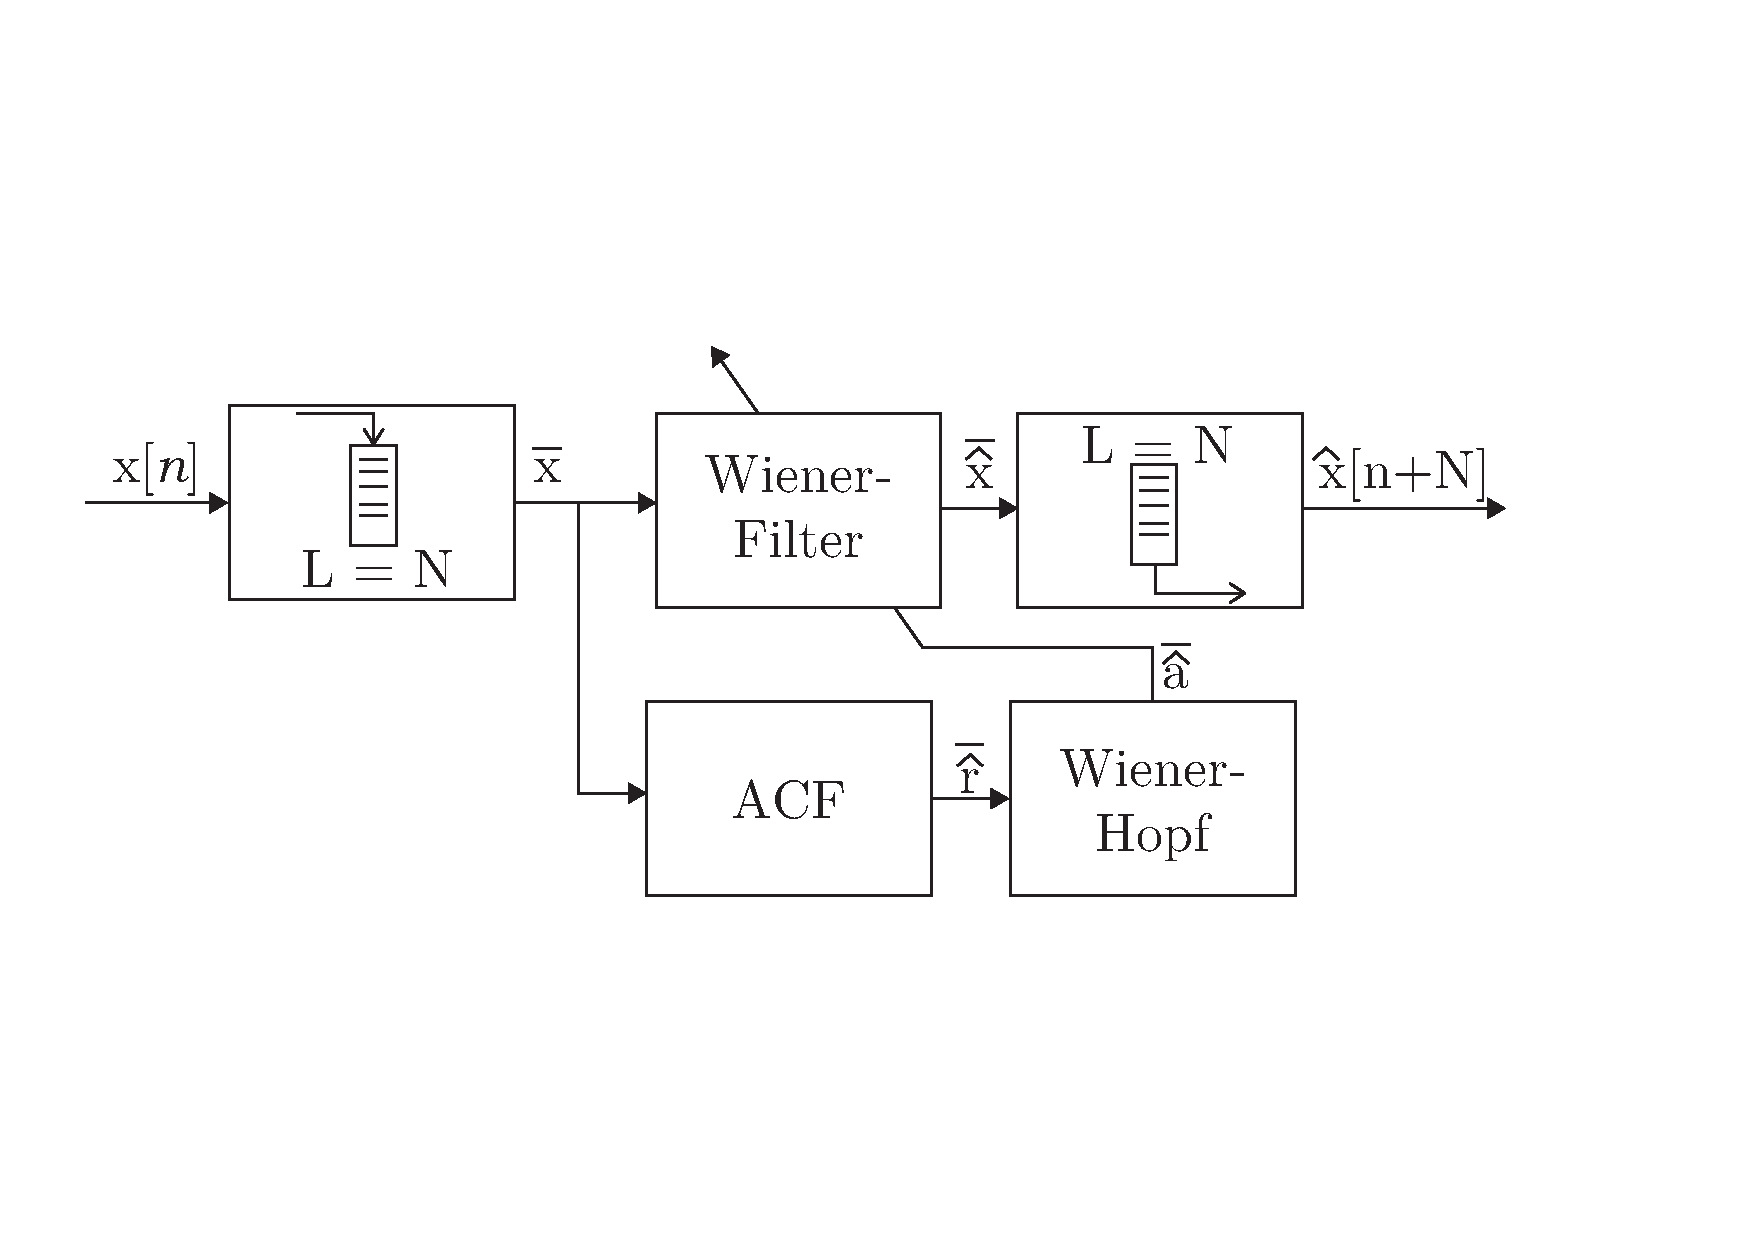
\includegraphics[width=\columnwidth]{figures/ArticleIllustrations/WienerHopf}
	\caption{Block diagram of linear prediction system.}
	\label{fig:APPLinearPredictionOverview}
\end{figure}
The system predicts $\hat{x}[n+P]$ by adapting linear prediction coefficients $\hat{\bar{a}}$, in a Wiener filter, determined using a framebased Auto Correlation Function (ACF) $\hat{r}_x[l]$ \cite{LinearPrediction}.

\begin{itemize} 
	\item $N$ is the framelength, that is the amount of previous samples stored and used for predicting the next sample. $\bar{x}$ in \autoref{fig:APPLinearPredictionOverview} has size $N$.
	\item $M$ is the order of the predictor, that is the amount of coefficients used for predicting the next sample. $\hat{\bar{a}}$ in \autoref{fig:APPLinearPredictionOverview} has size $M$.
	\item $O$ is the overlap, that is the amount of samples to be reused, when calculating the new ACF. A new ACF and new LPCs are estimated for each $N-O$ samples.
	\item $P$ determines the how many samples will be predicted. 
	\item $W$ is a window used for weighting the samples in the current frame when calculating the ACF. 
\end{itemize}


\subsection{Auto Correlation estimation}
The full autocorrelation would be an infinite time series, which would be impossible to calculate and it would not be useful as speech is not Wide Sense Stationary through infinite time. The short time stationarity of speech is used by only estimating the ACF for a short time frame determined by N/fs. The ACF is estimated using \autoref{eq:Appnonrecursive}.
\begin{equation}\label{eq:Appnonrecursive}
%%r_x[l,m] = \sum^{m}_{n=m-N+1+\left| l\right|} x_l[n]w_l[m-n]
\hat{r}_x[l] = \sum^{N}_{n=\left| l\right|} x_l[n]w_l[N-n]
\end{equation}
Where: l is the lag, $x_l[n]=x[n]x[n-l]$ and $w_l[n]=w[n]w[n+l]$. w is a window that can be applied to emphasize ?SOMETHING?. Some experimenting has been made using different windows. It was found that a Hamming window yielded best performance, but a rectangular window yielded almost similar results while saving a computations, as multiplying all samples by one can be omitted. A Barnwell window is proposed by \cite{speech}, but has been found to yield poorer results than both other windows.   


check the where - also in article\\\\
We claim something about 50-400 LPC in article\\
Is the WF equation not allready cascaded? Or not really. A sum over p is missing?\\
We lack a new CP\\
We lack a journal on measuring performance of ANC headphones\\
We lack HP and CP in article.\\


\subsection{ Wiener Hopf - Finding the Linear Prediction Coefficients}
 The Linear Prediction Coefficients (LPCs) are determined using \autoref{eq:normal}, known as the Wiener-Hopf equation.
\begin{equation}\label{eq:normal}
\hat{R}  \bar{a} = -\bar{\hat{r}}_x
\end{equation}
Where; $\hat{R}$ is the covariance matrix $\hat{C}_{xx}$, $\bar{\hat{a}}$ is the LPCs $\bar{\hat{a}} = [\hat{a}_0 , \hat{a}_1, \dotsc, \hat{a}_{N-1}]^T$ and $\bar{\hat{r}}_x$ is the ACF, $\bar{\hat{r}}_x = [\hat{r}_x[1] , \hat{r}_x[2], \dotsc, \hat{r}_x[N]]^T$. \autoref{eq:normal} can be rewritten as shown in \autoref{eq:normal2} yielding the LPCs directly.  
\begin{equation}\label{eq:normal2}
\bar{\hat{a}} = \hat{-R^{-1}} \bar{\hat{r}}_x
\end{equation}
Calculating $\hat{R}^{-1}$ is computationally heavy, therefore to estimate the LPCs the Levinson-Durbin method is used. 

\subsubsection{Levinson-Durbin}
Levinson-Durbin is a method which can be used to find the estimated LPCs of a problem, recursively. It is characterized by being power efficient, as it does not directly invert a matrix, but rather estimates it.
The algorithm takes the coefficients of the ACF in order to compute the RCs, which lastly yields the LPCs. The algorithm can be seen below3:\\\\
The coefficient order, $l$ is initialized to 0, which means the predictor for order 0 is found first:
\begin{equation}\label{LDInit}
	J_0=R[0]
\end{equation}
The algorithm works recursively, and the next step iterates for a total number of the prediction order, $M$ to compute RCs for each $l$.
\begin{equation}\label{LDStep1}
	k_l=\frac{1}{J_{l-1}} \left ( R[l] + \sum_{i=1}^{l-1} a_i^{(l-1)}R[l-i]   \right) 
\end{equation}
The LPC are then likewise calculated iteratively, from the already found RCs: 
\vspace{-0mm}
\begin{equation}\label{LDStep2_1}
	a_l^{(l)} = -k_1,
\end{equation}
\vspace{-10mm}
\begin{equation}\label{LDStep2_2}
a_i^{(l)} = a_i^{(l-1)} - k_l a_{l-i}^{(l-1)} ; \hspace{10mm} i = 1,2,\dotsc,l-1
\end{equation}
Lastly a minimizer for the mean-squared predictor is computed, for the $l$'th order computation:
\begin{equation}\label{LDStep2}
	J_1 = J_{l-1} (1-k_l^2)
\end{equation}
This gives the LPCs:
\begin{equation}
	a_i = a_i^{M}; \hspace{10mm} i = 1,2 \dotsc , M
\end{equation}


\subsection{Wiener filter}
A Wiener filter is used in cascade, where $\hat{x}[n+2]$ is estimated using $\hat{x}[n+1]$ and $x[n]$ up until $\hat{x}[n+P]$. 
\begin{equation}\label{eq:AppPredictor}
\hat{x}[n+p] =- \sum^{M-1}_{i=1}\hat{a}_i[n]x[(n+p)-i]
\end{equation}
The Wiener filter resembles an FIR filter, where the previous inputs are used in combination with the LPCs to predict the next sample. 

\subsection{Prediction Gain}
The Prediction Gain (PG) is an objective measure of the performance of a predictor measured in dB. 
\begin{equation}\label{eq:App_PG}
PG = 10 log_{10}\bigg(\frac{\sigma^2_x}{\sigma^2_\varepsilon}\bigg) = 10 log_{10}\bigg(\frac{E\{x^2[n]\}}{E\{\varepsilon^2[n]\}}\bigg)
\end{equation}
As seen in \autoref{eq:App_PG} the PG is calculated based on a ratio between the variance of the signal to be predicted $\sigma^2_x$ and the variance of the error of the predictor $\sigma^2_\varepsilon$. The PG value yields an estimate of the performance of the predictor, however it is necessary to also listen to the predicted signal, as it might be distorted. PG is used as the performance indicator, while searching for optimum parameters for the predictor.  


%\begin{figure}[H]
%	\tikzsetnextfilename{BasisCompare}
%	% This file was created by matlab2tikz.
%
%The latest updates can be retrieved from
%  http://www.mathworks.com/matlabcentral/fileexchange/22022-matlab2tikz-matlab2tikz
%where you can also make suggestions and rate matlab2tikz.
%
\definecolor{mycolor1}{rgb}{0.00000,0.44700,0.74100}%
\definecolor{mycolor2}{rgb}{0.85000,0.32500,0.09800}%
%
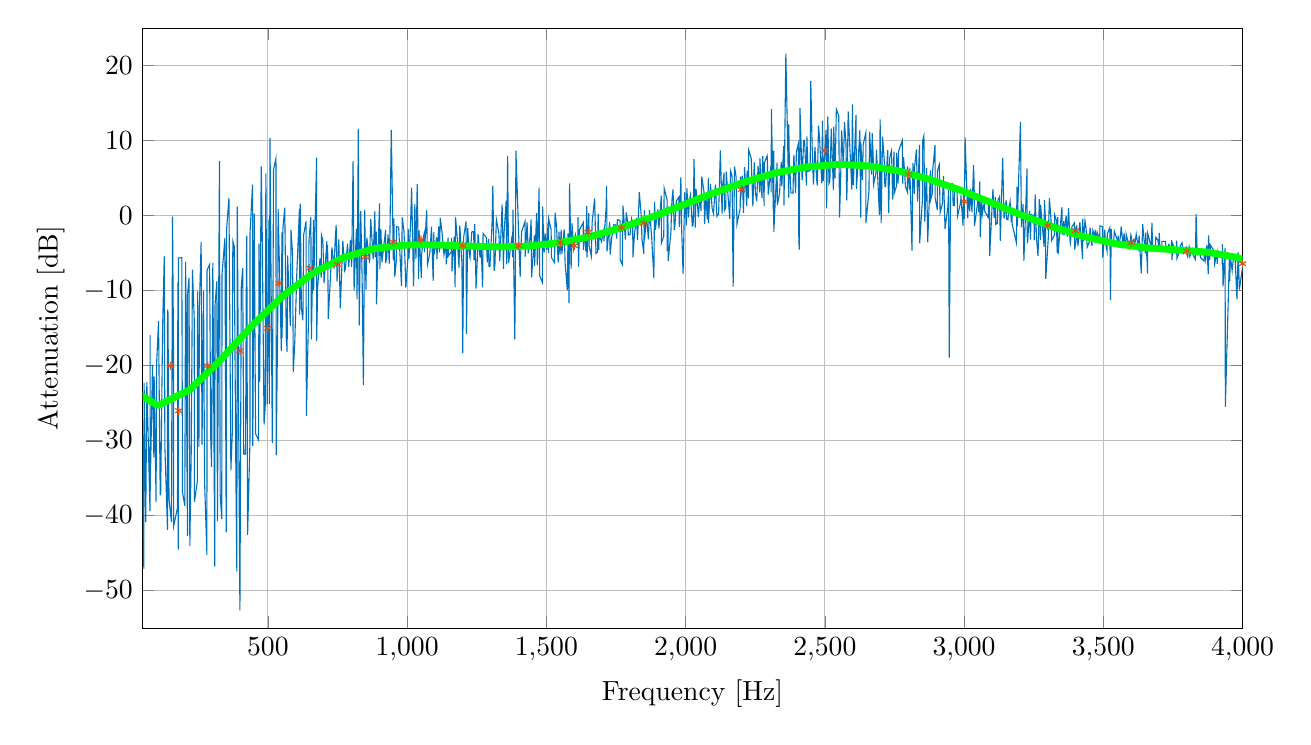
\begin{tikzpicture}

\begin{axis}[%
width=5.5in,
height=3in,
at={(1.011in,0.642in)},
scale only axis,
xmin=50,
xmax=4000,
xlabel={Frequency [Hz]},
xmajorgrids,
ymin=-55,
ymax=25,
ylabel={Attenuation [dB]},
ymajorgrids,
axis background/.style={fill=white},
title style={font=\bfseries},
%title={Basic ANC},
legend style={at={(0.03,0.03)},anchor=south west,legend cell align=left,align=left,draw=white!15!black}
]
\addplot [color=mycolor1,solid]
  table[row sep=crcr]{%
49.9997916675347	-29.3241740940108\\
54.5997725009479	-47.0972952166704\\
55.5997683342986	-22.2966757621044\\
61.3997441677326	-40.847752328958\\
65.3997275011354	-22.1719704886903\\
76.7996800013333	-39.3998614126295\\
77.1996783346736	-15.9156565027211\\
77.3996775013437	-36.7559392281124\\
85.7996425014896	-19.8973032005664\\
90.5996225015729	-32.2196008904446\\
91.5996183349236	-21.4174710501654\\
98.5995891683785	-38.1713171312877\\
100.39958166841	-19.7735873830439\\
107.399552501865	-14.0663920043817\\
113.399527501969	-37.2637520507453\\
115.199520002	-36.8566125769386\\
122.199490835455	-14.6188727983712\\
127.999466668889	-5.43389879100408\\
130.19945750226	-30.9168236323296\\
139.599418335757	-41.8746171369856\\
139.799417502427	-12.5144148985636\\
141.399410835788	-12.9705827311721\\
144.999395835851	-37.788263786232\\
153.799359169337	-40.834690737493\\
157.599343336069	-0.111384906346875\\
160.999329169462	-16.8982750611751\\
161.399327502802	-41.4415419511108\\
175.599268336382	-38.9138611404026\\
176.799263336403	-8.87492026385666\\
178.399256669764	-44.5320366816079\\
178.799255003104	-5.64613507564902\\
190.999204169983	-5.58273487362221\\
193.599193336694	-36.8881144770682\\
201.79915917017	-38.6696657291293\\
204.599147503552	-6.13895945467813\\
211.399119170337	-42.6718585724622\\
211.599118337007	-10.5070917171116\\
216.999095837101	-8.29267406187074\\
219.799084170483	-44.0139422171356\\
224.999062503906	-31.0264235788448\\
229.199045003979	-7.18027750436166\\
235.599018337424	-13.7316011658981\\
236.399015004104	-38.146207448713\\
246.998970837621	-35.3188853561676\\
247.598968337632	-10.0807155998943\\
252.398948337715	-30.8226187614988\\
254.198940837747	-12.0569056681469\\
260.398915004521	-3.47669173818617\\
263.598901671243	-30.505608646063\\
268.998879171337	-9.98299718061581\\
272.798863338069	-35.565233127251\\
281.198828338215	-45.2288026839322\\
281.398827504885	-7.28746060018329\\
290.798788338382	-6.50146263154113\\
294.998770838455	-29.7370920529928\\
297.798759171837	-33.4734554844638\\
302.39874000525	-6.24958704490318\\
309.398710838705	-46.7603375925864\\
310.198707505385	-11.9513547053816\\
316.99867917217	-8.71718934178258\\
318.798671672201	-40.7258278321247\\
326.198640838996	7.3268017704389\\
328.598630839038	-37.0670114142839\\
334.398606672472	-40.4448212745009\\
335.398602505823	-7.80492555817579\\
345.79855917267	-2.94574692413614\\
350.398540006083	-42.2072203373986\\
350.398540006083	-42.2072203373986\\
351.798534172774	-1.81801926681195\\
360.19849917292	2.39087221541965\\
367.198470006375	-33.9311139465229\\
372.398448339799	-28.9030372417408\\
374.19844083983	-3.37842338523715\\
379.198420006583	-4.07136473771895\\
385.398394173358	-35.6906721328368\\
388.59838084008	-47.4679354938989\\
390.198374173441	1.20247772278072\\
399.598335006937	-52.6197324261479\\
404.598314173691	-9.44394811287022\\
409.598293340444	-6.97749347386653\\
413.398277507177	-31.7927679419801\\
419.798250840622	-31.7718036951768\\
422.998237507344	-6.19152949077383\\
424.398231674035	-2.67962747422349\\
427.198220007417	-42.5456859210715\\
435.798184174233	-30.0421035588441\\
435.998183340903	-2.27466731141314\\
444.998145841059	4.14361413300346\\
445.79814250774	-30.6992176931151\\
450.998120841163	0.294952529760848\\
455.798100841246	-29.066421819533\\
466.598055841434	-29.8964279315369\\
468.198049174795	-3.7206830586117\\
470.598039174837	-22.1186663656859\\
476.198015841601	6.57042411803743\\
479.798000841663	-2.61010919970026\\
486.397973341778	-27.8346861682261\\
490.397956675181	-25.5595598930096\\
492.797946675222	5.64271560393513\\
497.797925841976	-25.1602407604569\\
503.99790000875	-0.530787025283434\\
505.397894175441	-25.0828884988035\\
507.597885008812	10.3575734588779\\
515.997850008958	-30.2955251907807\\
520.397831675701	6.11902727524473\\
528.997795842517	7.66373607324351\\
529.997791675868	-31.9214255127619\\
535.397769175962	-13.9107126039144\\
536.797763342653	0.888194327996841\\
548.397715009521	-18.0497558117509\\
550.397706676222	-2.21620417136463\\
551.197703342903	-16.2880657367016\\
553.797692509615	-1.78849213996894\\
560.597664176399	1.07084966585503\\
566.197640843163	-16.3021274915352\\
569.197628343215	-18.1810145375042\\
570.797621676576	-5.30498630961261\\
580.797580010083	-14.6965144129622\\
583.197570010125	-1.9319621037121\\
588.597547510219	-5.04787848654333\\
591.397535843601	-20.8484234426637\\
596.797513343694	-16.6725222786221\\
603.997483343819	-7.64608478309659\\
613.397444177316	0.917325819396537\\
614.197440843996	-13.1787215574767\\
616.397431677368	1.61657009791314\\
620.397415010771	-12.3541017669947\\
625.797392510864	-13.9404367679815\\
628.397381677576	-2.58910281446478\\
637.197345011062	-0.748014591023891\\
638.197340844413	-26.6891030201943\\
645.597310011208	-14.3740522497179\\
647.59730167791	-3.34660625298435\\
654.397273344694	-0.143954355464409\\
656.197265844726	-16.4751940385757\\
663.997233344861	-0.546780451740125\\
664.397231678201	-9.9312745035135\\
674.997187511719	7.74852612363824\\
675.197186678389	-16.6789970982129\\
678.797171678451	-9.48647715093702\\
687.197136678597	-5.67818480437094\\
691.59711834534	-8.23575650984339\\
692.597114178691	-2.61813553101317\\
697.397094178774	-3.28543171490804\\
701.797075845517	-8.96546298789319\\
711.997033345694	-3.35320426557944\\
712.997029179045	-6.67099518188366\\
714.597022512406	-3.9332503519175\\
716.997012512448	-13.7434873701032\\
726.196974179274	-7.11703881667595\\
729.996958346007	-4.2341581465599\\
737.596926679472	-7.03832663863284\\
741.396910846205	-3.52292636530628\\
745.196895012937	-1.22203819512391\\
748.39688167966	-8.74956914928326\\
754.796855013104	-3.13980180614639\\
759.996833346528	-12.3443101444171\\
759.996833346528	-12.3443101444171\\
769.196795013354	-3.34446749188618\\
769.196795013354	-3.34446749188618\\
775.796767513469	-7.31963428486907\\
778.39675668018	-7.09439635522689\\
785.996725013646	-3.73441651585069\\
790.196707513719	-6.8434327757567\\
796.396681680493	-3.22130901094141\\
796.396681680493	-3.22130901094141\\
800.796663347236	-6.85238777560907\\
805.99664168066	7.27839577812701\\
809.596626680722	-9.95591175658863\\
817.996591680868	-1.7286878461877\\
820.39658168091	-11.1110938053613\\
824.796563347653	11.5825887182255\\
827.996550014375	-14.6352989199316\\
833.396527514469	0.600095650984105\\
838.396506681222	-8.05212862909868\\
842.996487514635	-22.5416018570788\\
847.596468348049	0.797668067402527\\
852.196449181462	-9.85220105971558\\
855.396435848184	-2.92109531769203\\
865.396394181691	-6.31426633889371\\
867.396385848392	-3.02980351137854\\
869.596376681764	-0.463335458358332\\
877.99634168191	-5.83023137919764\\
884.196315848684	0.623870130729278\\
885.796309182045	-5.53284169522101\\
889.196295015437	-2.12469083509225\\
889.996291682118	-11.8155099760317\\
900.996245848976	1.65620812163564\\
902.196240848996	-7.08679145620987\\
905.796225849059	-1.78207828965839\\
909.596210015792	-6.22498187546604\\
922.796155016021	-1.90329941468685\\
922.996154182691	-6.31002667850858\\
926.596139182753	-5.59365681045154\\
931.596118349507	-2.48214121766796\\
935.79610084958	-6.37290269914697\\
938.396090016292	-2.28301461295833\\
943.196070016375	11.4571110162751\\
950.59603918317	-5.96735616229173\\
952.396031683201	-0.344764176181075\\
955.796017516594	-8.11783405081304\\
961.195995016687	-6.00133992742413\\
962.595989183378	-1.45412487234474\\
969.595960016833	-1.5222146256688\\
974.595939183587	-5.32089486851557\\
979.79591751701	-9.39524198696103\\
982.395906683722	-0.216601096093727\\
988.995879183837	-2.17801978653238\\
995.395852517281	-9.59372455035722\\
1002.99582085075	-5.55343370663929\\
1003.79581751743	-1.71372306083192\\
1006.59580585081	-5.70626870071678\\
1012.39578168424	-1.09204984553057\\
1016.19576585098	3.7500230292906\\
1023.19573668443	-9.43457451873946\\
1027.79571751784	1.55082417383113\\
1031.59570168458	-5.80019282271598\\
1036.19568251799	4.20185231201237\\
1041.39566085141	-8.46836930868676\\
1042.7956550181	-1.94411991097551\\
1051.19562001825	-8.30251615412882\\
1052.1956158516	-5.14993008369898\\
1058.99558751839	-2.74909941004907\\
1060.99557918509	-2.39221088164256\\
1062.39557335178	-4.84354604622631\\
1070.19554085191	0.742609472909075\\
1073.39552751864	-6.47720445533786\\
1081.79549251878	-4.93151534853916\\
1087.59546835222	-1.46098107950758\\
1093.59544335232	-8.6701278690242\\
1095.99543335236	-2.15355667343774\\
1096.99542918571	-5.18703101111181\\
1105.99539168587	-2.8791189710174\\
1106.99538751922	-5.82892017608917\\
1113.39536085266	-1.41218254521028\\
1115.99535001937	-4.88035977325409\\
1119.1953366861	-0.282539014990738\\
1125.1953116862	-2.15774248902961\\
1132.39528168633	-5.20323544362584\\
1138.99525418644	-3.51172844672924\\
1140.5952475198	-6.4977387430928\\
1147.39521918659	-2.89353461882889\\
1147.79521751993	-5.39183644539548\\
1159.19517002012	-4.77768205920589\\
1159.99516668681	-2.97050004921022\\
1161.19516168683	-7.42559623057559\\
1169.19512835363	-2.80163157176809\\
1172.39511502035	-9.54531385828542\\
1173.99510835372	-0.207335505136459\\
1179.99508335382	-2.93433868592474\\
1186.39505668726	-6.91986159067789\\
1189.19504502065	-1.32076467652315\\
1196.79501335411	-6.29832075006795\\
1199.79500085416	-18.2827602570548\\
1203.19498668756	-2.84078069355655\\
1211.5949516877	-0.763448474128174\\
1213.19494502106	-15.7371791037655\\
1217.59492668781	-1.66957934398899\\
1222.79490502123	-4.98266095200954\\
1225.79489252128	-5.60141079464232\\
1232.3948650214	-2.14820287153047\\
1239.19483668818	-2.10693284611761\\
1240.19483252153	-5.91739055191772\\
1242.99482085491	-1.11597577911787\\
1247.59480168833	-9.72038745156936\\
1251.59478502173	-6.29958728011832\\
1254.79477168845	-2.45385435714524\\
1261.79474252191	-5.56357927817138\\
1265.79472585531	-4.08440950513175\\
1271.1947033554	-9.51762127406799\\
1272.79469668876	-2.33903742948455\\
1284.39464835563	-2.9077499969742\\
1287.79463418902	-6.22831636914444\\
1292.79461335578	-3.08841254855069\\
1293.79460918913	-6.75985895729325\\
1297.39459418919	-6.76722593944862\\
1304.79456335599	-1.28974503420468\\
1307.79455085604	4.02471614913219\\
1312.39453168945	-7.34092099427075\\
1315.3945191895	-6.48580695451016\\
1320.59449752293	-0.526223138070294\\
1329.59446002308	-2.3741922132676\\
1332.99444585648	-6.07341075658075\\
1333.39444418982	-5.49364278779424\\
1341.19441168995	1.51187762625619\\
1345.99439169003	-7.09749488947148\\
1347.99438335674	-2.36545340133729\\
1355.79435085687	2.01148614819249\\
1357.39434419023	-6.48020487699884\\
1360.9943291903	7.98047160335482\\
1364.19431585702	-6.32700227538147\\
1376.99426252391	-2.6478123935262\\
1378.79425502394	-5.55132970477845\\
1380.19424919063	0.825165683263617\\
1386.59422252407	-16.4749354467509\\
1387.99421669076	-11.7862074757684\\
1390.79420502415	8.68746529588781\\
1399.7941675243	-1.70447463889048\\
1405.99414169108	-8.19895027413721\\
1406.99413752443	-5.89859376392457\\
1411.1941200245	-2.14288206301829\\
1423.39406919138	-0.787872757122735\\
1424.39406502473	-5.46210769694524\\
1424.39406502473	-5.46210769694524\\
1430.79403835817	-0.887108309794973\\
1435.19402002492	-5.00724420734326\\
1441.9939916917	-2.69849188293735\\
1445.39397752509	-0.492525946574747\\
1446.99397085845	-8.25524381711676\\
1457.19392835863	-2.62707084138844\\
1457.79392585864	-6.68365677502283\\
1464.99389585877	0.345546386334745\\
1467.59388502548	-6.58723074915647\\
1473.99385835892	3.73194847306008\\
1475.99385002562	-7.99035010265201\\
1485.79380919246	-8.91395754746086\\
1486.59380585914	1.252514385427\\
1491.99378335924	-4.92640849688864\\
1495.99376669264	-2.38163816737074\\
1501.19374502606	-4.56281987290683\\
1506.39372335949	-0.808000331756134\\
1507.99371669285	-4.99747950710065\\
1508.39371502619	-0.41707813897531\\
1517.19367835967	-1.91097901937221\\
1518.19367419302	-5.56306096498421\\
1529.59362669322	-6.26713316612505\\
1531.39361919325	0.400854426259594\\
1536.39359836001	-1.30370367525169\\
1542.39357336011	-6.24304908640811\\
1545.39356086016	-2.12657089970173\\
1548.99354586023	-5.19085682639188\\
1553.1935283603	-1.89174416425691\\
1555.79351752701	-5.09674418463758\\
1563.99348336049	-1.81452635231029\\
1567.39346919388	-6.32698226569328\\
1575.39343586068	-9.95751954494547\\
1577.79342586073	-2.36729466053099\\
1581.39341086079	-11.6197996444249\\
1583.39340252749	4.31912502428711\\
1588.99337919425	-7.0689340732765\\
1592.19336586098	-1.02745825580291\\
1597.59334336107	-4.33841837832241\\
1604.39331502785	-2.5595794662349\\
1612.99327919467	-3.76337991628125\\
1613.79327586135	-0.180353666593952\\
1615.79326752805	-6.8025279670405\\
1618.39325669476	-1.90771893582891\\
1632.59319752834	-0.906417222240246\\
1632.79319669501	-4.55004921134671\\
1633.79319252836	-1.99173052260635\\
1641.5931600285	-4.74628090444867\\
1644.99314586189	1.26691628476784\\
1645.99314169524	-5.56159798267388\\
1652.39311502869	0.32980813498891\\
1653.79310919538	-4.05807222389001\\
1661.59307669551	-5.39381960656581\\
1664.3930650289	-0.891825539908396\\
1673.39302752905	2.31047730039889\\
1678.19300752914	-5.02291368164343\\
1683.59298502923	-4.8643543310335\\
1686.19297419594	0.248041107976148\\
1688.39296502931	-4.55608701966884\\
1689.19296169599	-2.45674873584422\\
1697.99292502948	-3.45170677835994\\
1706.19289086295	-1.98070485857017\\
1706.99288752964	-3.40073135470567\\
1714.5928558631	1.14695517004881\\
1716.39284836313	3.98255959761469\\
1717.79284252982	-4.75355562039743\\
1727.39280252999	-0.866651483065353\\
1728.99279586335	-5.19935199376018\\
1734.39277336344	-3.01062992785667\\
1742.19274086358	-1.19670872186364\\
1748.59271419702	-1.23424014576393\\
1752.19269919709	-3.04366740424218\\
1752.19269919709	-3.04366740424218\\
1755.19268669714	-0.515457264483156\\
1764.79264669731	-0.661052175547719\\
1764.99264586398	-5.83757792848482\\
1772.59261419744	-6.50415678470406\\
1775.19260336415	1.33475327677798\\
1783.79256753097	-3.17213366611498\\
1786.79255503102	0.449392578105023\\
1792.59253086445	-0.980026810799395\\
1794.39252336449	-2.58887747403034\\
1800.59249753126	-2.51044398281354\\
1806.19247419802	-0.42095983750772\\
1809.99245836476	-1.11345023547837\\
1810.99245419811	-5.54485167459096\\
1816.59243086487	-2.37605523584001\\
1823.99240003167	-0.293558459841075\\
1827.39238586506	-3.25051994892028\\
1833.7923591985	3.15291901078395\\
1841.59232669864	-0.387970990537919\\
1842.99232086533	-2.95612250824042\\
1849.99229169878	-5.06814946151935\\
1851.99228336549	0.749990244484972\\
1852.79228003217	-3.15680248210694\\
1859.79225086562	-0.0523316473918733\\
1866.39222336574	-3.13466253506397\\
1870.39220669914	0.742423225455651\\
1870.39220669914	0.742423225455651\\
1878.19217419927	-2.83199306443478\\
1885.99214169941	-8.27076397929251\\
1888.59213086612	1.87543837232288\\
1888.59213086612	1.87543837232288\\
1891.3921191995	-1.89460810510063\\
1900.19208253299	0.849920069384262\\
1904.39206503306	-1.67397114445416\\
1912.79203003321	2.67016198753165\\
1913.19202836655	-3.65013435852991\\
1921.59199336669	-2.72518341275074\\
1922.99198753339	3.67896854637241\\
1933.5919433669	2.11338952595738\\
1933.99194170024	-4.73583983707456\\
1936.19193253361	1.24733178046103\\
1937.59192670031	-6.01007154107379\\
1947.19188670047	-2.26420282031997\\
1950.79187170053	1.93539817764746\\
1954.79185503394	3.4957144177255\\
1959.39183586735	-1.90565549225272\\
1961.59182670072	-1.34741229910018\\
1966.99180420082	1.99171115697692\\
1975.59176836763	2.4630877380735\\
1977.59176003433	-1.46990968199592\\
1982.99173753443	5.13903315965989\\
1985.39172753447	-1.20717095737503\\
1990.99170420123	-7.74759400293082\\
1996.79168003467	3.10456892014595\\
2002.79165503477	-1.29412251388447\\
2004.5916475348	3.70948393134576\\
2010.39162336824	-0.201504422595303\\
2013.9916083683	2.06878396213873\\
2017.59159336836	2.75615036055539\\
2023.99156670181	-1.3607191202884\\
2027.19155336853	-1.22759989294484\\
2030.39154003525	7.54742131460224\\
2034.59152253532	-1.59573875638153\\
2037.59151003537	3.57359516935575\\
2046.19147420219	-0.183852928919653\\
2050.7914550356	2.77602291019761\\
2055.39143586902	0.644168510007918\\
2058.1914242024	5.19803759057554\\
2065.99139170253	3.18850517966555\\
2068.19138253591	-1.11709147777415\\
2072.59136420265	2.78184782807201\\
2078.19134086941	-0.499322521686547\\
2081.79132586948	5.03214394481968\\
2082.19132420282	-0.973982003499203\\
2089.39129420294	4.23931601446273\\
2095.19127003637	1.01985171195431\\
2100.19124920313	0.262008014596938\\
2107.19122003658	4.13979299712049\\
2107.19122003658	4.13979299712049\\
2112.39119837001	-0.083327760854027\\
2118.59117253678	0.250867043818117\\
2124.79114670356	8.72374156383687\\
2131.191120037	0.229980336896992\\
2132.99111253703	3.97331718571557\\
2138.19109087045	5.75164853217855\\
2139.59108503715	0.70949083007641\\
2143.99106670389	1.07813277465071\\
2145.99105837059	5.87983781628507\\
2158.59100587081	-0.436912315879264\\
2161.39099420419	5.98384980742234\\
2166.79097170428	5.30865521827686\\
2170.79095503769	-9.45209505439692\\
2170.79095503769	-9.45209505439692\\
2175.79093420444	6.53790343774094\\
2181.3909108712	5.16552505629832\\
2184.39089837126	-1.10112752413591\\
2195.99085003812	0.955989668596588\\
2197.39084420482	5.20937247178375\\
2198.1908408715	2.378165770134\\
2203.59081837159	5.33744320623573\\
2207.79080087166	0.397917942803315\\
2211.79078420507	6.48905213665932\\
2219.99075003854	1.26714822657727\\
2220.79074670522	5.98878466601294\\
2225.59072670531	2.31161391928412\\
2226.39072337199	8.77469847945735\\
2235.59068503881	7.65279800061553\\
2241.59066003892	1.25236450279823\\
2246.59063920567	7.0974258711926\\
2250.79062170574	3.0596360868225\\
2255.59060170583	1.94290668178319\\
2260.19058253924	6.62705442025271\\
2266.59055587268	3.0973854511097\\
2266.79055503935	7.67846896693997\\
2274.19052420615	2.34952614995847\\
2277.1905117062	7.94542915550166\\
2282.19049087295	1.28033573394122\\
2282.39049003962	7.00605575677604\\
2292.99044587314	7.98650368166187\\
2296.99042920654	2.83388202346736\\
2306.39039004004	6.66857605552718\\
2307.19038670672	3.10977331230539\\
2308.19038254007	14.2052449906333\\
2315.19035337353	0.391183499448725\\
2316.39034837355	8.64917265235708\\
2316.79034670689	-2.13995622346657\\
2328.59029754043	7.07077748985118\\
2329.39029420711	1.42152258179718\\
2337.39026087391	2.98563518414983\\
2343.39023587402	7.18764109622069\\
2345.59022670739	3.91688320837871\\
2352.1901992075	9.27737893683312\\
2353.39019420752	1.37990204285289\\
2359.99016670764	21.6163399802344\\
2370.39012337449	2.39744422689284\\
2370.59012254116	12.1811695467796\\
2372.19011587452	7.89829352091724\\
2378.39009004129	3.05034323245143\\
2385.59006004142	3.02171562384818\\
2388.79004670814	8.15873472568609\\
2394.99002087491	3.04511850486204\\
2397.7900092083	8.49100817663748\\
2404.78998004175	9.57267844925525\\
2406.58997254178	-3.29276417594273\\
2408.38996504181	-4.50310729837841\\
2410.78995504185	14.3394112576203\\
2418.58992254199	4.72255489817717\\
2423.78990087541	9.98928455076802\\
2427.18988670881	10.0442917205258\\
2433.98985837559	4.06397954587856\\
2435.58985170895	10.5748457367366\\
2439.18983670901	5.90752588299342\\
2447.38980254249	6.0336882015191\\
2449.58979337586	17.9407469495686\\
2454.18977420927	9.63290745282528\\
2458.98975420936	4.13913811388395\\
2464.58973087612	9.13084727243471\\
2470.58970587623	4.86849901763445\\
2472.7896967096	4.04075416867375\\
2477.38967754301	12.0091388688335\\
2481.18966170974	10.2718234726293\\
2488.98962920988	4.34404305486408\\
2491.58961837659	12.675859813977\\
2494.38960670997	4.61827453563986\\
2504.58956421015	11.480444603671\\
2506.38955671018	0.995088651387692\\
2510.58953921025	13.2254212595638\\
2514.989520877	4.30223009697934\\
2517.98950837705	4.5533318640472\\
2523.18948671047	11.6269770965728\\
2530.78945504394	3.41164152613544\\
2532.18944921063	11.8714879334302\\
2536.58943087737	4.97458165254912\\
2541.38941087745	14.2017579551924\\
2549.98937504427	13.3248906919883\\
2552.78936337765	-0.235145632593874\\
2556.58934754438	4.4957522206435\\
2560.38933171112	11.3848435974752\\
2566.38930671122	6.45390552915662\\
2570.58928921129	12.5206000189122\\
2575.98926671139	9.64768042314859\\
2578.78925504477	2.04217650168066\\
2580.78924671147	5.39292096099546\\
2583.78923421152	13.920234936393\\
2596.98917921175	3.46724709273827\\
2598.18917421177	11.0565241828143\\
2599.18917004512	14.8409702258079\\
2602.18915754518	4.11615412944533\\
2611.98911671201	13.4196672706878\\
2613.3891108787	3.58119041609129\\
2618.38909004546	6.36433066399983\\
2625.78905921225	11.4352783647006\\
2628.78904671231	-0.262892922450285\\
2629.38904421232	9.76504865895489\\
2635.18902004575	4.7364641872597\\
2637.78900921246	9.52364280721116\\
2647.38896921263	11.0803170855119\\
2647.5889683793	-0.955687464642008\\
2658.38892337949	3.2771543564831\\
2660.78891337953	11.2208680619111\\
2667.98888337965	5.49470164422024\\
2669.98887504635	11.0131110710763\\
2673.58886004642	7.9665999299268\\
2674.98885421311	4.12037851252325\\
2683.18882004658	5.64967366691493\\
2685.38881087995	8.80043745343789\\
2695.98876671347	0.0957687525982055\\
2698.58875588018	12.8605373120182\\
2702.18874088025	-0.991139968167824\\
2707.188720047	10.5505445094879\\
2713.38869421377	7.46019416391482\\
2715.58868504715	3.87533818524453\\
2717.98867504719	3.87459354374186\\
2725.78864254732	8.74382115714469\\
2729.38862754739	0.34342380070761\\
2732.78861338078	7.69437621661808\\
2739.38858588089	8.66293055271188\\
2743.58856838097	2.15399417546503\\
2748.18854921438	8.53728468956428\\
2749.78854254774	3.04136169218705\\
2757.18851171453	3.92740592439259\\
2757.98850838122	8.40025862839733\\
2763.18848671464	4.28459316810654\\
2764.98847921467	8.62176344483803\\
2777.98842504823	10.0123954814934\\
2779.58841838159	4.26760446824015\\
2782.78840504831	7.81949393152592\\
2789.5883767151	3.87991255842267\\
2796.78834671522	3.12118190142624\\
2796.98834588189	6.56334360861432\\
2804.38831504869	3.4767186219761\\
2805.18831171537	6.40104302167177\\
2812.9882792155	-4.66800867365144\\
2816.18826588223	7.05549558717757\\
2821.38824421565	2.91716822188146\\
2821.58824338232	6.27757690769333\\
2828.98821254911	8.84074232783032\\
2833.18819504919	1.89435028339731\\
2839.7881675493	9.46130308327621\\
2840.58816421598	-3.67638454110934\\
2851.1881200495	2.56395980711099\\
2851.38811921617	10.0160261379226\\
2855.78810088291	10.6708903446706\\
2858.98808754964	-0.76978090483059\\
2865.18806171641	6.35669166778039\\
2869.38804421648	-3.51759511194843\\
2879.18800338332	6.03067649126663\\
2879.58800171666	2.06653447138893\\
2885.58797671676	2.89014509642117\\
2886.18797421677	5.63539657171251\\
2895.58793505027	9.40898700753186\\
2896.18793255028	2.37670916635824\\
2904.18789921709	0.750434746824666\\
2904.38789838376	6.01500268176023\\
2910.7878717172	6.80949354010334\\
2913.98785838392	0.426736019764354\\
2921.78782588406	1.52512773479054\\
2926.1878075508	5.28313371687365\\
2926.1878075508	5.28313371687365\\
2931.5877850509	-1.74442347417459\\
2941.78774255107	1.08240045563408\\
2944.38773171778	3.4918468164305\\
2946.78772171783	-18.9171432282808\\
2951.78770088458	4.11944208762738\\
2958.78767171803	4.25589986794874\\
2960.78766338474	1.35657013996386\\
2964.58764755147	1.35004989078842\\
2966.18764088483	3.67163359242741\\
2974.98760421832	3.04794125508982\\
2976.58759755168	-0.0340561791152932\\
2988.18754921854	1.87931225953462\\
2988.38754838521	2.77397820908721\\
2996.18751588535	-1.30186312077819\\
2998.18750755205	3.52466242208545\\
3000.78749671876	-0.414096669033231\\
3003.78748421882	10.4144800946103\\
3013.18744505231	-0.318371543460057\\
3015.58743505235	3.33370634013467\\
3020.38741505244	0.588652267383713\\
3023.58740171916	3.56615515225639\\
3028.38738171924	0.468088473129033\\
3033.98735838601	6.74570913771423\\
3036.18734921938	4.12776131243808\\
3037.3873442194	-1.3726099211271\\
3051.98728338632	2.66051953201126\\
3052.787280053	0.508066517819059\\
3056.18726588639	4.54844230985475\\
3058.18725755309	-2.84531819757784\\
3062.78723838651	2.53343591344851\\
3065.58722671989	0.248986002111975\\
3071.98720005333	1.67809697599991\\
3074.1871908867	0.599895534379423\\
3086.58713922025	-0.258321984362166\\
3088.58713088695	2.01215244877814\\
3091.58711838701	1.67761272581025\\
3091.98711672035	-5.36003338264205\\
3103.58706838721	3.53012445341764\\
3108.18704922063	-0.294167275710557\\
3112.18703255403	2.48383317947822\\
3113.78702588739	-1.15504068918984\\
3119.18700338749	-1.03432037668769\\
3121.7869925542	2.06931297658922\\
3127.38696922096	2.53303251314145\\
3130.18695755434	-3.36383597574303\\
3138.58692255449	7.73009876715362\\
3143.58690172124	-0.38169580990106\\
3151.18687005471	2.09424919669926\\
3152.38686505473	-0.444068580766738\\
3157.38684422148	-0.534119680070424\\
3160.78683005487	0.779526625593629\\
3165.38681088829	1.86342826355511\\
3169.78679255503	-0.895372957447652\\
3171.9867833884	0.581168705276026\\
3172.38678172174	-1.05651087019512\\
3187.98671672201	-3.61950503938543\\
3189.98670838871	3.85365182260168\\
3191.18670338874	-1.42631354267226\\
3193.38669422211	1.77336417634053\\
3202.38665672226	12.5052494859168\\
3205.98664172233	-1.55466353419287\\
3211.98661672243	1.53820377178716\\
3214.78660505581	-6.01151612378015\\
3226.18655755601	6.28822547745772\\
3226.58655588935	-2.52381453520464\\
3227.98655005604	-3.65837550931236\\
3234.78652172283	0.596983647640745\\
3238.78650505623	-3.19112396798004\\
3240.18649922292	0.162917086197951\\
3250.78645505644	0.0298902095160477\\
3252.18644922313	-3.25053192601138\\
3255.18643672318	2.8463995591434\\
3259.98641672326	-2.95512895245154\\
3265.58639339003	-5.36985535464459\\
3270.18637422344	2.1997785500537\\
3274.18635755684	-3.24960903681516\\
3274.78635505685	1.44783867233316\\
3287.38630255707	-4.16144749337799\\
3288.38629839042	2.08408087694361\\
3291.98628339049	-0.298664927311236\\
3293.38627755718	-8.41166849348651\\
3302.38624005733	-2.998000648967\\
3306.38622339074	2.3436503428721\\
3311.9862000575	-0.424093406936334\\
3314.38619005754	-3.31916474764064\\
3324.78614672439	-2.54711956543332\\
3324.98614589106	0.129920919343287\\
3331.58611839117	-0.623296127430979\\
3334.38610672456	-4.93601846677256\\
3336.38609839126	-0.167171485682221\\
3337.58609339128	-5.14115642812747\\
3351.38603589152	1.14614447069866\\
3352.1860325582	-2.52944677916731\\
3358.1860075583	-0.718179934513729\\
3358.98600422498	-2.62613423494315\\
3366.58597255845	-0.0137160797522589\\
3370.38595672518	-2.78534262108202\\
3375.18593672526	1.01547788090615\\
3380.38591505869	-3.2839257961594\\
3381.58591005871	-3.62128562260011\\
3387.38588589214	-1.45076848310539\\
3395.98585005896	-0.970566109733375\\
3397.18584505898	-4.51733283554783\\
3403.38581922575	-3.03765745149406\\
3404.58581422577	-1.28867919176695\\
3408.98579589252	-4.05304210390886\\
3415.7857675593	-0.850549973066627\\
3425.58572672614	-5.77248153133967\\
3425.98572505948	-0.435798741513305\\
3428.58571422619	-3.42592087294797\\
3434.18569089295	-0.677984907954345\\
3437.98567505969	-1.61779525026164\\
3442.18565755976	-4.19018409112622\\
3449.9856250599	-3.48827930363605\\
3452.38561505994	-1.58966355040287\\
3459.18558672672	-4.00895924566485\\
3462.58557256011	-1.96534018058397\\
3470.18554089358	-2.86672963111318\\
3470.58553922692	-1.84382354682496\\
3472.98552922696	-3.16510999231051\\
3477.78550922704	-2.1819556703454\\
3487.18547006054	-3.28328014070138\\
3487.58546839388	-1.34803909456262\\
3497.18542839405	-1.46590106855153\\
3498.1854242274	-5.62789847855138\\
3504.98539589418	-1.85024259330526\\
3507.78538422757	-3.66865887800298\\
3513.585360061	-4.70241757206556\\
3514.38535672768	-2.41339919511874\\
3523.58531839451	-1.5992791893295\\
3525.58531006121	-11.2151381054398\\
3528.58529756126	-1.77670913928083\\
3530.38529006129	-3.75219829064152\\
3536.78526339474	-3.59712908414495\\
3539.78525089479	-2.06829970493009\\
3553.38519422836	-3.6060939138504\\
3553.7851925617	-2.65618771249954\\
3555.18518672839	-4.29562237169057\\
3561.58516006183	-2.69317588194599\\
3564.18514922854	-1.42169593649718\\
3570.38512339532	-3.80203070519363\\
3574.58510589539	-2.34811415832944\\
3578.78508839546	-4.16193859054637\\
3581.58507672885	-4.07778221393435\\
3582.18507422886	-2.50159765339261\\
3593.9850250624	-4.20828116982565\\
3598.98500422915	-2.5656409218257\\
3601.78499256253	-3.00726941425453\\
3602.58498922921	-3.81144119856427\\
3609.78495922934	-3.17407926616276\\
3613.18494506273	-3.80768301371036\\
3618.18492422948	-2.44014725538603\\
3625.58489339628	-4.23481310267566\\
3628.784880063	-2.64505142067569\\
3636.18484922979	-7.68380417003242\\
3636.18484922979	-7.68380417003242\\
3641.38482756322	-1.13567071188244\\
3650.78478839671	-5.00881446106851\\
3652.18478256341	-2.2426072184253\\
3659.18475339686	-7.73231112252069\\
3659.38475256353	-2.3525279655667\\
3664.38473173028	-3.02086930062085\\
3671.98470006375	-4.3103346444741\\
3674.58468923046	-0.951723315102069\\
3677.18467839717	-4.52222904883557\\
3686.58463923067	-4.09243714131264\\
3688.78463006404	-2.86575192565137\\
3695.7846008975	-3.24798279974021\\
3699.18458673089	-4.1455194845242\\
3700.98457923092	-2.30120108949924\\
3703.18457006429	-4.42582848408444\\
3709.98454173108	-4.41408669725944\\
3710.38454006442	-3.42999202456697\\
3722.78448839796	-3.42613143589576\\
3726.38447339803	-4.54758783353697\\
3729.38446089808	-4.35377662418056\\
3735.58443506485	-3.83575557032447\\
3744.58439756501	-4.68365415616316\\
3745.18439506502	-3.25069068889054\\
3746.58438923171	-5.92946670465099\\
3749.58437673176	-3.79629120270287\\
3760.58433089862	-4.8571872487028\\
3763.58431839867	-3.33104195691771\\
3763.58431839867	-3.33104195691771\\
3763.98431673201	-5.71726246927168\\
3774.7842717322	-4.67851548902563\\
3776.98426256557	-3.99363650934097\\
3782.58423923234	-3.57752825761241\\
3787.78421756576	-4.99340261480366\\
3797.5841767326	-4.25269872676366\\
3797.98417506594	-4.8460931585632\\
3803.18415339936	-5.45766931827049\\
3808.58413089945	-4.10865611060426\\
3809.38412756613	-4.21793662832876\\
3810.58412256616	-5.42745098503129\\
3818.18409089962	-4.53859605362138\\
3818.78408839963	-4.95822948263446\\
3830.58403923317	-5.81891529816664\\
3833.18402839988	0.232409233030503\\
3836.3840150666	-4.22934221338319\\
3839.18400339999	-5.09985764670532\\
3846.58397256678	-4.58310162191157\\
3848.58396423348	-5.55821453442038\\
3861.58391006704	-6.03335639627119\\
3862.78390506706	-4.56728197062453\\
3867.18388673381	-5.82600530388364\\
3871.78386756722	-3.92417497311081\\
3876.78384673397	-7.76899591805933\\
3877.98384173399	-2.62546752217597\\
3882.18382423407	-5.89556291235624\\
3884.78381340078	-3.92134823314714\\
3899.58375173437	-4.81194810366703\\
3900.18374923438	-6.3810611713092\\
3908.18371590118	-4.90470244027167\\
3908.98371256786	-6.42842237666074\\
3909.3837109012	-6.06460005353734\\
3910.7837050679	-4.71507373266932\\
3925.98364173483	-5.03059198369534\\
3927.38363590152	-6.54297289594903\\
3927.58363506819	-3.78648846630457\\
3929.98362506823	-9.37636938325671\\
3937.38359423502	-4.32970026467942\\
3938.1835909017	-25.4934656969645\\
3952.98352923529	-5.34025288692338\\
3953.78352590198	-8.70857405790679\\
3956.38351506869	-5.50786723886067\\
3962.58348923546	-7.31315776255171\\
3963.78348423548	-6.79911179057289\\
3968.78346340224	-5.26752047480428\\
3973.18344506898	-5.54311707024782\\
3979.78341756909	-11.1479414962738\\
3984.18339923584	-4.84649929586972\\
3988.58338090258	-9.84100657153822\\
4000.18333256945	-6.8138602098318\\
};
%\addlegendentry{Basic ANC Response};

\addplot[only marks,mark=asterisk,mark options={},mark size=1.5000pt,color=mycolor2] plot table[row sep=crcr]{%
0	-20\\
40	-30\\
150	-20\\
180	-26\\
284	-20\\
400	-18\\
500	-15\\
540	-9\\
650	-7\\
750	-6.5\\
850	-5.5\\
950	-3.5\\
1050	-3.2\\
1200	-4\\
1400	-4\\
1550	-3.6\\
1600	-4\\
1650	-2.2\\
1770	-1.6\\
1850	-1\\
2200	3.5\\
2500	8.7\\
2800	5.5\\
3000	1.9\\
3300	-1.3\\
3400	-2\\
3600	-3.6\\
3800	-4.7\\
4000	-6.4\\
4100	-7.2\\
};
%\addlegendentry{Fit};

\addplot [color=green,solid,line width=2.5pt]
  table[row sep=crcr]{%
0	-22.958549087386\\
0	-22.958549087386\\
101.19957833509	-25.232470937237\\
110.599539168587	-25.2165251965534\\
221.199078337174	-23.1623790102402\\
221.199078337174	-23.1623790102402\\
331.79861750576	-19.1488463067431\\
331.79861750576	-19.1488463067431\\
442.398156674347	-14.6995153429527\\
442.398156674347	-14.6995153429527\\
552.997695842934	-10.7099411344863\\
552.997695842934	-10.7099411344863\\
663.597235011521	-7.61603125486959\\
663.597235011521	-7.61603125486959\\
774.196774180108	-5.53293493890101\\
774.196774180108	-5.53293493890101\\
884.796313348694	-4.36752227525031\\
884.796313348694	-4.36752227525031\\
995.395852517281	-3.90739527326011\\
995.395852517281	-3.90739527326011\\
1053.19561168495	-3.85994508458175\\
1105.99539168587	-3.88922758884026\\
1216.59493085445	-4.04908469426077\\
1216.59493085445	-4.04908469426077\\
1327.19447002304	-4.1572312765686\\
1335.99443335653	-4.15799757352527\\
1437.79400919163	-4.03978764927149\\
1437.79400919163	-4.03978764927149\\
1548.39354836022	-3.58945196185164\\
1548.39354836022	-3.58945196185164\\
1658.9930875288	-2.76735999158888\\
1658.9930875288	-2.76735999158888\\
1769.59262669739	-1.59800930209114\\
1769.59262669739	-1.59800930209114\\
1880.19216586598	-0.159029552851305\\
1880.19216586598	-0.159029552851305\\
1990.79170503456	1.43256425593495\\
1990.79170503456	1.43256425593495\\
2101.39124420315	3.03614381913955\\
2101.39124420315	3.03614381913955\\
2211.99078337174	4.50391805898016\\
2211.99078337174	4.50391805898016\\
2322.59032254032	5.69686036982877\\
2322.59032254032	5.69686036982877\\
2433.18986170891	6.49905579162423\\
2433.18986170891	6.49905579162423\\
2543.7894008775	6.82955632807854\\
2560.58933087779	6.83551622508348\\
2654.38894004608	6.65097762592279\\
2654.38894004608	6.65097762592279\\
2764.98847921467	5.97421523151886\\
2764.98847921467	5.97421523151886\\
2875.58801838326	4.85880364127955\\
2875.58801838326	4.85880364127955\\
2986.18755755184	3.40858636237849\\
2986.18755755184	3.40858636237849\\
3096.78709672043	1.76251020031114\\
3096.78709672043	1.76251020031114\\
3207.38663588902	0.0805019900333797\\
3207.38663588902	0.0805019900333797\\
3317.9861750576	-1.47546901267084\\
3317.9861750576	-1.47546901267084\\
3428.58571422619	-2.76489486268055\\
3428.58571422619	-2.76489486268055\\
3539.18525339478	-3.69640556301791\\
3539.18525339478	-3.69640556301791\\
3649.78479256336	-4.25908039136955\\
3649.78479256336	-4.25908039136955\\
3760.38433173195	-4.55671069849422\\
3760.38433173195	-4.55671069849422\\
3870.98387090054	-4.84418596136065\\
3870.98387090054	-4.84418596136065\\
3981.58341006912	-5.56502987405797\\
3981.58341006912	-5.56502987405797\\
4092.18294923771	-7.38896825853325\\
4092.18294923771	-7.38896825853325\\
};
%\addlegendentry{Poly};

\end{axis}
\end{tikzpicture}%
%	\label{Fig:BasisCompare}
%	\caption{Text here.}
%\end{figure}

%\begin{figure}[H]
%	\tikzsetnextfilename{LPCompare}
%	% This file was created by matlab2tikz.
%
%The latest updates can be retrieved from
%  http://www.mathworks.com/matlabcentral/fileexchange/22022-matlab2tikz-matlab2tikz
%where you can also make suggestions and rate matlab2tikz.
%
\definecolor{mycolor1}{rgb}{0.00000,0.44700,0.74100}%
\definecolor{mycolor2}{rgb}{0.85000,0.32500,0.09800}%
%
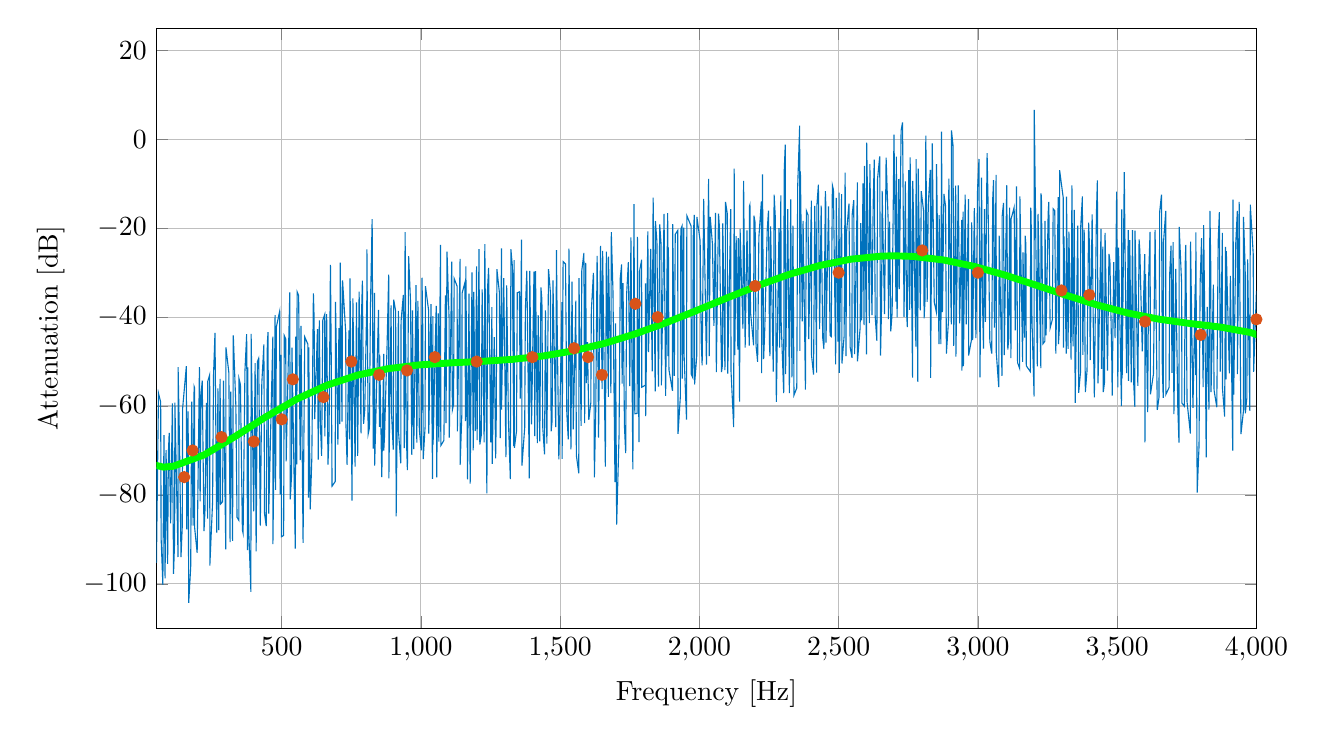
\begin{tikzpicture}

\begin{axis}[%
width=5.5in,
height=3in,
at={(1.011in,0.642in)},
scale only axis,
xmin=50,
xmax=4000,
xlabel={Frequency [Hz]},
xmajorgrids,
ymin=-110,
ymax=25,
ylabel={Attenuation [dB]},
ymajorgrids,
axis background/.style={fill=white},
title style={font=\bfseries},
%title={LP ANC},
legend style={at={(0.03,0.03)},anchor=south west,legend cell align=left,align=left,draw=white!15!black}
]
\addplot [color=mycolor1,solid]
  table[row sep=crcr]{%
49.9997916675347	-73.7200111331179\\
50.1997908342049	-95.2926508023547\\
57.599760001	-57.1392881458429\\
65.3997275011354	-59.1244831162125\\
66.9997208344965	-89.7686933486108\\
73.1996950012708	-100.22538502824\\
77.1996783346736	-66.5466970224496\\
81.1996616680764	-98.7618103836172\\
84.7996466681389	-69.9215561017927\\
90.3996233349028	-95.4944425813552\\
92.9996125016146	-70.7667647135462\\
95.9996000016666	-66.0472628035094\\
101.19957833509	-86.4015465681852\\
107.399552501865	-59.3910780752362\\
111.599535001937	-97.7485890834033\\
115.59951833534	-90.0868052662447\\
116.399515002021	-59.2512188927865\\
127.799467502219	-93.9715078241451\\
127.999466668889	-51.268478202642\\
133.199445002312	-68.7370942858639\\
138.399423335736	-93.9857368214841\\
142.799405002479	-87.2853100332051\\
144.39939833584	-60.4238729413436\\
157.599343336069	-51.0123416702896\\
159.199336669431	-87.77764315879\\
163.999316669514	-61.1943623497921\\
165.999308336215	-104.315568524028\\
173.19927833634	-96.2523455913086\\
176.799263336403	-59.0177108739009\\
181.999241669826	-86.8882554159833\\
185.399227503219	-55.570000115396\\
187.19922000325	-55.9120576242528\\
187.39921916992	-87.3993389703308\\
196.399181670076	-93.0531841291544\\
204.599147503552	-51.2560574030613\\
206.999137503594	-81.470174998486\\
210.399123336986	-57.4073576417924\\
214.599105837059	-54.2712098591294\\
220.999079170503	-88.1634991957591\\
224.599064170566	-83.3564840101337\\
229.599043337319	-59.3028063092394\\
233.999025004062	-85.3284276715764\\
234.599022504073	-54.4434708199148\\
241.398994170858	-52.9769912265293\\
241.998991670868	-95.914139501812\\
251.798950837705	-81.641784696759\\
255.198936671097	-53.0195062716279\\
260.398915004521	-43.5717444466473\\
266.798888337965	-88.4613313896887\\
270.998870838038	-56.0507959290352\\
273.79885917142	-87.9340480713999\\
278.798838338174	-53.9105179252308\\
280.998829171545	-82.0170082345442\\
287.59880167166	-81.5605729576709\\
290.798788338382	-54.3009989119129\\
299.198753338528	-92.2796456440064\\
299.798750838538	-46.795782676568\\
310.198707505385	-52.5039355820795\\
313.998691672118	-82.6245487749923\\
314.598689172128	-90.6267604572013\\
316.99867917217	-56.7393717152716\\
323.598651672285	-90.322067478861\\
326.198640838996	-44.1102366492513\\
335.398602505823	-59.9916083074054\\
339.598585005896	-85.0468462519558\\
346.19855750601	-85.7262759861167\\
346.598555839351	-53.818209462795\\
351.798534172774	-55.1805683274047\\
358.798505006229	-87.8999817147648\\
361.398494172941	-88.6320205164519\\
367.998466673056	-52.1091609846414\\
374.19844083983	-43.8506315066793\\
377.198428339882	-92.4360897030129\\
378.198424173233	-51.303131568488\\
381.598410006625	-87.9113997424251\\
389.39837750676	-101.832512303818\\
390.198374173441	-43.777614239586\\
399.398335840267	-83.7022017600132\\
404.598314173691	-50.3395152473686\\
408.198299173753	-92.6884087344134\\
412.798280007167	-50.0237838696066\\
417.39826084058	-49.2687634933025\\
423.198236674014	-86.9349910128883\\
423.198236674014	-86.9349910128883\\
428.598214174108	-54.8195981730049\\
435.998183340903	-46.1454532802304\\
438.398173340944	-84.2089089274372\\
444.398148341049	-87.0290926848717\\
448.398131674451	-45.7817479943701\\
450.998120841163	-43.3651984286218\\
453.398110841205	-84.2288311841148\\
468.198049174795	-44.3936371515867\\
468.398048341465	-91.0491263794713\\
471.798034174858	-73.4414024613408\\
476.198015841601	-39.5306363029458\\
477.998008341632	-78.8429645671053\\
480.997995841684	-42.1565803247863\\
492.797946675222	-38.6688495077476\\
494.197940841913	-79.860151097462\\
497.397927508635	-48.5102178441652\\
499.397919175337	-89.3972119945195\\
506.997887508802	-89.1399223388318\\
509.197878342174	-44.1576395216752\\
514.397856675597	-44.9142198421242\\
515.997850008958	-72.4715755055534\\
528.997795842517	-34.4404079386317\\
530.797788342549	-80.9833674533757\\
535.597768342632	-75.3957371718996\\
536.797763342653	-46.8652625048514\\
548.797713342861	-92.102425875096\\
550.397706676222	-44.3640977886048\\
554.397690009625	-73.1181488754401\\
555.197686676305	-34.2855905266492\\
560.797663343069	-35.121418171588\\
566.397640009833	-72.1981168093903\\
569.197628343215	-41.9719868295395\\
576.797596676681	-90.7861781448937\\
577.997591676701	-79.80887015997\\
582.797571676785	-44.4761342934371\\
594.197524176983	-46.1326041640856\\
596.197515843684	-80.6179064111992\\
596.997512510365	-46.8288214799295\\
602.397490010458	-83.2454904989437\\
608.197465843892	-71.6907296929247\\
613.797442510656	-34.6573301301217\\
616.397431677368	-40.2332186925458\\
618.59742251074	-62.9657455721106\\
628.397381677576	-42.7245089968928\\
631.197370010958	-72.0724390853433\\
635.197353344361	-40.7228978656776\\
638.597339177753	-63.507538578206\\
643.397319177837	-71.2236064077294\\
647.59730167791	-40.6640915601626\\
654.397273344694	-39.4283757100873\\
654.797271678035	-66.8403757551865\\
661.397244178149	-39.3461844997971\\
666.197224178233	-73.1900033449723\\
669.997208344965	-66.2337486478548\\
674.997187511719	-28.2471057379194\\
678.597172511781	-54.2515809505897\\
680.797163345153	-78.0474461970754\\
692.197115845351	-76.9870795392146\\
693.197111678701	-36.5554042975494\\
701.797075845517	-68.6783863323391\\
705.39706084558	-42.4633090173954\\
708.597047512302	-64.0636593190982\\
710.197040845663	-27.7308580039371\\
716.597014179108	-63.4941399884135\\
718.597005845809	-31.7636298034702\\
729.996958346007	-43.5792751131246\\
730.596955846017	-63.9162276770814\\
734.79693834609	-73.2360162708563\\
741.396910846205	-42.9697419625559\\
743.796900846246	-67.5039617668552\\
745.196895012937	-31.2709335221925\\
752.596864179733	-81.3077701694043\\
755.596851679785	-35.811963680359\\
763.59681834659	-73.6306520165619\\
768.596797513344	-36.6767475248746\\
772.796780013417	-71.2075949691823\\
777.99675834684	-34.2902169501287\\
784.996729180295	-66.1489419973031\\
785.996725013646	-41.0799710351087\\
789.796709180378	-31.8005138658485\\
793.996691680451	-64.0315922613741\\
798.196674180524	-60.976009197155\\
805.596643347319	-36.2428294344209\\
805.99664168066	-24.7480798123159\\
810.396623347403	-66.3340450714721\\
814.996604180816	-64.961084604753\\
818.596589180878	-38.0447562282026\\
824.796563347653	-17.9622086560826\\
828.796546681055	-69.599865157946\\
833.396527514469	-34.5721373772155\\
833.796525847809	-73.4054562067635\\
847.596468348049	-38.3525480692672\\
850.996454181441	-64.7152516025514\\
851.796450848121	-48.4449764992347\\
859.396419181587	-75.997160047984\\
866.396390015042	-48.2477929597173\\
866.596389181712	-70.0398972112281\\
869.196378348424	-66.7950438973733\\
878.39634001525	-46.3262800403992\\
884.196315848684	-30.4233139780739\\
884.796313348694	-76.2687808085208\\
892.7962800155	-37.3676847402239\\
894.796271682201	-62.1216710279031\\
900.596247515635	-69.8158205627851\\
902.196240848996	-36.078618624068\\
909.196211682451	-38.6291070766045\\
910.996204182483	-84.8234544073006\\
919.196170015958	-38.5885393866865\\
919.596168349299	-65.8585833592318\\
927.596135016104	-72.8752646686924\\
928.596130849455	-40.948609673221\\
936.79609668293	-35.0208289600669\\
940.196082516323	-69.4833661361442\\
943.196070016375	-20.897282432285\\
946.796055016437	-65.1439552096596\\
951.396035849851	-74.4453780328545\\
955.796017516594	-26.3033493744657\\
962.595989183378	-36.4918812775437\\
967.195970016792	-70.9805866207606\\
969.595960016833	-38.4726268837656\\
974.195940850246	-69.7180587086718\\
982.395906683722	-32.8077449940865\\
985.195895017104	-68.2336928400952\\
988.995879183837	-36.3559175678894\\
994.19585751726	-65.3518448063376\\
1001.19582835072	-69.9639810413965\\
1003.79581751743	-31.1443128473432\\
1006.39580668414	-41.8881434071291\\
1008.19579918417	-71.932279801854\\
1014.79577168428	-64.7842242808723\\
1016.19576585098	-33.0337979158526\\
1027.79571751784	-38.6295667288778\\
1028.19571585118	-66.2348961451213\\
1036.19568251799	-37.0837770480774\\
1041.59566001808	-76.3721915279064\\
1042.7956550181	-39.8015971143036\\
1043.59565168478	-68.6802158970359\\
1054.79560501831	-37.4785063429796\\
1056.59559751834	-76.0701239692572\\
1062.19557418511	-39.1822756840932\\
1064.19556585181	-68.0147977266529\\
1070.19554085191	-23.7260981438686\\
1071.39553585193	-68.9072745631323\\
1082.39549001879	-67.7377168525352\\
1087.79546751889	-35.0977745894953\\
1089.99545835226	-63.8489493354397\\
1093.59544335232	-25.2771766064773\\
1100.99541251911	-40.2463943266695\\
1101.7954091858	-67.1332358206547\\
1110.59537251928	-27.5431621774506\\
1112.79536335265	-60.9002990367052\\
1117.1953450194	-59.6593588000766\\
1119.1953366861	-31.3041716827357\\
1129.99529168628	-33.0707492659076\\
1130.79528835297	-65.6819981110192\\
1140.5952475198	-26.9130231210607\\
1140.79524668647	-73.2706664421254\\
1146.79522168658	-61.95627262145\\
1147.79521751993	-34.6051908702237\\
1158.19517418677	-32.1704260610218\\
1159.79516752014	-63.403384832594\\
1161.19516168683	-28.5577660624464\\
1167.3951358536	-76.534405889116\\
1172.39511502035	-34.741451504629\\
1176.7950966871	-77.4875690712241\\
1183.39506918721	-29.9569326887348\\
1187.59505168728	-69.9813923131446\\
1189.79504252066	-34.3061952399445\\
1194.79502168741	-65.6602196755932\\
1199.79500085416	-28.5890289090081\\
1201.59499335419	-67.6621225261057\\
1208.59496418765	-24.7128704476395\\
1211.39495252103	-68.6818522928919\\
1216.39493168778	-66.7033887052524\\
1219.79491752118	-33.7553416800474\\
1226.9948875213	-68.2051532313772\\
1229.39487752134	-23.5530565896447\\
1236.79484668814	-79.6658932307515\\
1239.19483668818	-33.5597520137213\\
1242.99482085491	-28.9476939192374\\
1250.79478835505	-68.1837314874029\\
1254.79477168845	-37.7550105116098\\
1255.99476668847	-72.9967936486834\\
1263.1947366886	-44.5052826563768\\
1268.19471585535	-71.7599994812361\\
1270.39470668872	-62.4983626202923\\
1272.79469668876	-29.2139795852669\\
1281.59466002225	-34.4205908951618\\
1284.79464668897	-67.2265841181828\\
1289.19462835572	-24.5104533654661\\
1289.39462752239	-60.8406397727385\\
1297.19459502252	-31.2443868419271\\
1305.19456168933	-71.4928696703821\\
1307.79455085604	-32.84867886007\\
1314.19452418948	-63.3006982851433\\
1320.99449585627	-76.4297932717365\\
1322.99448752297	-24.713352221831\\
1328.39446502306	-28.6011442187182\\
1333.39444418982	-69.0378422439871\\
1334.39444002317	-27.1521993047123\\
1335.59443502319	-69.431488155733\\
1342.99440418998	-65.7209845562009\\
1345.99439169003	-34.5096600541026\\
1353.5943600235	-34.3106151134626\\
1356.39434835688	-58.3520987502113\\
1360.9943291903	-22.5582277866145\\
1362.79432169033	-73.3928148887285\\
1372.59428085716	-64.8712166878356\\
1374.9942708572	-38.2893698538358\\
1380.19424919063	-29.5712258474175\\
1387.79421752409	-68.8816427556069\\
1388.99421252411	-76.295071041347\\
1390.79420502415	-29.6043751286373\\
1397.19417835759	-64.120661063592\\
1405.99414169108	-29.7649405852614\\
1408.79413002446	-66.7812229415904\\
1411.39411919117	-29.6763428276673\\
1417.99409169128	-68.3392048136258\\
1420.99407919134	-39.539417428515\\
1426.79405502477	-67.9321010837901\\
1430.79403835817	-33.3008886807241\\
1434.39402335824	-36.1493658181964\\
1437.39401085829	-64.8048464710732\\
1443.79398419173	-70.8970243167994\\
1446.99397085845	-38.5021447132358\\
1452.19394919188	-68.4630034435284\\
1458.19392419198	-29.195156264336\\
1464.99389585877	-34.584323309055\\
1467.59388502548	-65.6940040638327\\
1470.99387085887	-63.3082535547965\\
1473.99385835892	-31.7274030092744\\
1483.99381669243	-64.7346062065332\\
1486.59380585914	-24.9411163844072\\
1489.19379502585	-41.5215028198486\\
1495.19377002596	-72.0148609619801\\
1497.593760026	-65.5155118036131\\
1506.39372335949	-36.6184778382164\\
1506.9937208595	-71.8964037781584\\
1510.39370669289	-27.5047052810628\\
1519.19367002637	-28.0512211683332\\
1523.79365085979	-61.5588379046053\\
1528.99362919321	-67.5156222762551\\
1531.39361919325	-24.5949804852449\\
1538.59358919338	-69.7777146956454\\
1542.39357336011	-32.0174885179188\\
1542.79357169345	-34.9013078713773\\
1546.99355419352	-65.2300487598124\\
1556.19351586035	-36.2806519378606\\
1557.99350836038	-71.0721720274603\\
1566.79347169387	-75.1272074763404\\
1567.39346919388	-31.221171906624\\
1575.19343669401	-64.4815891711882\\
1577.59342669406	-29.5477166594578\\
1585.19339502752	-25.5599660055181\\
1587.79338419423	-63.8513050459115\\
1591.59336836097	-27.8232818466269\\
1593.99335836101	-54.8393301702203\\
1597.99334169441	-45.6185379628129\\
1602.79332169449	-63.1251514361105\\
1609.99329169462	-59.2726528225779\\
1611.79328419465	-38.6586368084568\\
1619.39325252811	-30.0375410950662\\
1622.79323836151	-76.0379667793653\\
1627.79321752826	-60.5574561596829\\
1632.59319752834	-26.2217551972362\\
1633.79319252836	-32.0866500480885\\
1637.79317586177	-67.1162053251802\\
1644.99314586189	-23.9472510749373\\
1650.59312252866	-56.2047730116419\\
1652.39311502869	-25.1010830943186\\
1658.9930875288	-56.7429474969889\\
1662.19307419552	-73.6477996837261\\
1665.79305919559	-25.2593987156878\\
1673.19302836238	-57.9714657750691\\
1673.39302752905	-26.3992179012566\\
1682.19299086254	-57.1066040075825\\
1683.59298502923	-20.8807731265887\\
1689.59296002933	-34.2686573457558\\
1696.79293002946	-77.1395402808099\\
1698.59292252949	-41.4201498604399\\
1702.79290502956	-86.7078470941728\\
1711.39286919638	-66.5915950040042\\
1715.79285086312	-31.1879885146011\\
1720.5928308632	-28.1473981007387\\
1722.39282336324	-54.9689558322694\\
1725.59281002996	-32.3645005111181\\
1730.79278836338	-64.5674782421178\\
1735.19277003012	-70.6147547380591\\
1738.59275586352	-34.8969522217215\\
1744.79273003029	-27.6080418016849\\
1749.99270836372	-55.5330453924182\\
1753.99269169712	-22.0798616578307\\
1760.99266253057	-74.2773557119591\\
1764.99264586398	-14.5505823218857\\
1767.99263336403	-61.7557011578671\\
1776.1925991975	-61.6599258250864\\
1777.39259419752	-21.9428791713081\\
1782.99257086429	-68.1314379054113\\
1785.79255919767	-29.3898581071911\\
1792.59253086445	-27.0929594973811\\
1792.99252919779	-55.7637233517929\\
1805.79247586468	-55.3357945803122\\
1806.19247419802	-32.38245931114\\
1806.9924708647	-62.2994040024741\\
1814.79243836484	-20.725314082295\\
1817.19242836488	-47.8705537422293\\
1824.99239586502	-24.6448064450478\\
1830.39237336511	-52.2110771096035\\
1833.7923591985	-13.0997310160992\\
1841.1923283653	-56.7228050198675\\
1841.99232503198	-18.3796878780483\\
1847.39230253207	-23.0521310656577\\
1852.19228253216	-52.3904201379695\\
1852.99227919884	-55.6120758506286\\
1857.39226086558	-19.1355469129994\\
1862.39224003233	-23.6466158835567\\
1863.39223586568	-55.3421909371689\\
1872.99219586585	-16.7999572563227\\
1878.59217253261	-57.7404817955813\\
1885.99214169941	-16.6167009481865\\
1887.19213669943	-48.7489685005393\\
1888.59213086612	-24.2823697975993\\
1890.59212253282	-51.8712630719019\\
1903.19207003304	-56.589824561217\\
1903.99206669972	-19.0606528416955\\
1909.79204253316	-53.2311206651043\\
1913.19202836655	-21.3713282512403\\
1921.99199170003	-20.5166526052868\\
1923.19198670006	-66.2823640173253\\
1931.39195253353	-57.9910500899881\\
1933.19194503356	-20.2127248080372\\
1937.59192670031	-19.5111879383179\\
1938.39192336699	-53.8586986372134\\
1943.79190086708	-19.8447882910522\\
1944.79189670043	-48.2700434625556\\
1953.59186003392	-63.0438566134729\\
1954.79185503394	-17.1805529620922\\
1970.19179086754	-19.5269486745775\\
1970.59178920088	-52.8318570488674\\
1975.99176670097	-53.5944930077117\\
1977.59176003433	-22.0978221093981\\
1981.59174336774	-17.0145055277942\\
1982.59173920109	-55.1565091231531\\
1990.39170670122	-48.7354786214488\\
1990.99170420123	-17.4730424596624\\
2002.5916558681	-22.8561020443824\\
2006.5916392015	-45.7179644405451\\
2009.79162586823	-50.8542183094909\\
2015.19160336832	-13.4233895018484\\
2017.59159336836	-21.7897518926178\\
2025.19156170183	-50.672138194399\\
2025.19156170183	-50.672138194399\\
2032.99152920196	-8.90964269111883\\
2035.391519202	-48.7908798095396\\
2038.7915050354	-17.436368193383\\
2046.7914717022	-23.6411486960704\\
2051.99145003562	-41.9733014059664\\
2057.59142670239	-16.5526490616013\\
2060.79141336911	-52.3653262224403\\
2061.79140920246	-46.5968570644606\\
2068.59138086925	-16.7072403227312\\
2071.5913683693	-19.5682039225137\\
2079.19133670276	-52.3647199843263\\
2082.59132253616	-50.8310697128905\\
2083.79131753618	-18.9320276456525\\
2091.59128503631	-51.9169622300737\\
2093.79127586968	-14.0959220117831\\
2099.99125003646	-16.729985090649\\
2101.59124336982	-52.7038198946623\\
2112.39119837001	-15.7064459873086\\
2113.39119420336	-52.0961147138697\\
2122.99115420352	-64.7501008961677\\
2124.79114670356	-6.58885067457105\\
2126.99113753693	-48.5661355904986\\
2131.79111753701	-21.7651892664766\\
2137.99109170378	-47.3185213561448\\
2139.59108503715	-22.2494273531567\\
2144.19106587056	-58.9995972709312\\
2145.99105837059	-20.1542764639144\\
2156.19101587077	-42.5606293149914\\
2158.59100587081	-9.34234358398256\\
2164.19098253757	-46.8431162639112\\
2170.79095503769	-20.4910854552827\\
2178.79092170449	-46.4270312293925\\
2179.59091837117	-15.0776940278515\\
2181.3909108712	-14.7021301143517\\
2183.39090253791	-38.8512790644415\\
2194.59085587143	-46.3529488944618\\
2195.79085087145	-17.158084116805\\
2199.99083337153	-18.7421829601359\\
2203.39081920492	-46.5110177464208\\
2208.99079587168	-50.0452622134685\\
2213.39077753843	-22.10173031867\\
2222.39074003858	-13.990086096533\\
2223.39073587193	-52.5856254740866\\
2226.39072337199	-7.86231176516326\\
2230.59070587206	-49.4730775332605\\
2234.59068920546	-42.8078017956012\\
2243.39065253895	-20.5586584087885\\
2247.99063337236	-16.0303110395414\\
2251.79061753909	-46.2468246824104\\
2253.19061170578	-48.7507104856612\\
2255.59060170583	-19.6014327561283\\
2265.19056170599	-52.2894698108494\\
2268.19054920605	-12.4272222777122\\
2272.39053170612	-17.402835945303\\
2276.19051587285	-59.0589527226107\\
2285.79047587302	-19.987726811842\\
2287.99046670639	-46.8679875379761\\
2292.39044837313	-12.6274133294662\\
2293.59044337315	-41.2089262020605\\
2302.59040587331	-57.0989371117127\\
2304.19039920667	-7.66755151065863\\
2308.19038254007	-1.20468425786153\\
2309.39037754009	-52.8169036812865\\
2317.19034504023	-15.7305113102046\\
2322.99032087366	-57.119708889218\\
2327.79030087375	-13.487699968115\\
2332.19028254049	-53.5420675211312\\
2335.79026754055	-19.3983130040977\\
2339.59025170728	-57.5566670238385\\
2349.59021004079	-55.9415938485894\\
2352.79019670751	-10.6784754882304\\
2359.99016670764	3.10432005675343\\
2360.59016420765	-47.6183182403257\\
2362.59015587435	-7.20912547481431\\
2369.39012754114	-40.9765811956144\\
2372.19011587452	-18.3318904982456\\
2378.9900875413	-48.2153884062368\\
2380.59008087466	-56.2996919609807\\
2383.99006670806	-16.0598057642254\\
2390.19004087483	-17.0745739882753\\
2392.3900317082	-44.9305131805698\\
2402.18999087504	-13.784796047544\\
2402.58998920838	-48.6033481497906\\
2409.7899592085	-52.9536258340475\\
2414.18994087525	-14.9800673306742\\
2420.78991337536	-52.5067156178668\\
2421.58991004204	-15.0493419984914\\
2427.18988670881	-10.187429774871\\
2431.58986837555	-42.6815237526058\\
2437.18984504231	-14.938749225493\\
2442.58982254241	-44.5506445115095\\
2446.98980420915	-47.1676063904472\\
2452.18978254257	-11.6568672922186\\
2454.18977420927	-15.4509773575118\\
2454.38977337594	-45.7560416334988\\
2463.58973504277	-15.0709222139792\\
2469.18971170953	-44.1059181161468\\
2473.18969504294	-44.3658925647042\\
2477.38967754301	-10.3291403775765\\
2481.18966170974	-11.3185631538996\\
2489.18962837655	-50.6251609605941\\
2491.18962004325	-13.175822176838\\
2497.78959254336	-45.5085255636275\\
2501.78957587677	-12.0171651227423\\
2502.18957421011	-52.5496691843657\\
2510.58953921025	-12.3440036207477\\
2511.78953421027	-50.4301505750091\\
2519.58950171041	-44.2381237242446\\
2523.18948671047	-7.47264141569057\\
2526.38947337719	-48.7893091672894\\
2528.3894650439	-20.903399727358\\
2536.98942921071	-14.4485333575226\\
2541.18941171078	-46.7442890526849\\
2547.7893842109	-49.1547833537437\\
2548.38938171091	-17.0287471980728\\
2553.98935837767	-13.7078555302199\\
2557.1893450444	-48.3441756368518\\
2567.38930254457	-9.68716190768348\\
2567.58930171124	-49.9471198689813\\
2577.18926171141	-42.3119499468642\\
2579.38925254478	-18.8361235197724\\
2582.5892392115	-40.705545262152\\
2587.38921921159	-9.91332738969533\\
2591.18920337832	-41.8279030581062\\
2592.58919754501	-6.00037195093727\\
2599.98916671181	-48.3684051601381\\
2600.58916421182	-0.744099588967814\\
2610.38912337865	-41.3653054020273\\
2611.98911671201	-5.55780626936835\\
2619.58908504548	-39.5499484065894\\
2623.98906671222	-14.3724079412623\\
2627.78905087895	-4.5725912458508\\
2631.18903671235	-39.9209297551857\\
2637.18901171245	-45.3394201371221\\
2639.58900171249	-8.89174248896834\\
2647.38896921263	-3.82772056961629\\
2650.38895671268	-48.6353411494935\\
2654.18894087941	-37.0325217679688\\
2656.18893254611	-11.5909358941903\\
2664.78889671293	-39.3491651605465\\
2670.38887337969	-4.12009750871864\\
2677.38884421315	-17.6908661842103\\
2678.58883921317	-40.4596598275034\\
2682.98882087991	-18.5293853407219\\
2687.18880337999	-43.1823304292471\\
2691.98878338007	-38.9987774876997\\
2698.58875588018	1.0484949881196\\
2705.78872588031	-36.5000278480554\\
2707.188720047	-3.87605691280335\\
2709.78870921371	-40.0733337209052\\
2715.58868504715	-8.97289000598577\\
2717.58867671385	-33.7134172617198\\
2724.18864921396	1.97855013426472\\
2729.38862754739	3.80830354575096\\
2734.78860504748	-39.9236657996513\\
2739.38858588089	-9.45308119781073\\
2743.98856671431	-39.2020766881751\\
2746.58855588102	-42.2325603850583\\
2751.58853504777	-6.92070182017113\\
2754.98852088116	-38.367038399229\\
2756.58851421452	-4.06870827143708\\
2765.38847754801	-53.6172385081668\\
2766.18847421469	-9.3600559201453\\
2777.38842754822	-46.6535167986647\\
2777.98842504823	-4.45539857196337\\
2784.188399215	-54.5945806969669\\
2785.58839338169	-6.60508164933722\\
2793.18836171516	-38.464224414865\\
2796.58834754855	-11.6765928956789\\
2805.18831171537	-16.2811578030601\\
2806.78830504873	-40.2813323185156\\
2810.38829004879	-35.8889832877712\\
2812.9882792155	0.821738654998458\\
2817.78825921559	-36.5674953244655\\
2821.78824254899	-14.6335824627383\\
2828.98821254911	-6.87475538641894\\
2830.18820754914	-53.6479289607853\\
2835.98818338257	-0.88834822641945\\
2843.18815338269	-36.6318668560355\\
2850.78812171616	-38.8483909790915\\
2851.38811921617	-5.58219482783809\\
2860.18808254966	-46.0778342445091\\
2860.78808004967	-17.0758839516629\\
2866.98805421644	-46.079034468195\\
2869.38804421648	1.73836858144841\\
2872.5880308832	-38.861418660846\\
2877.9880083833	-12.2822434563085\\
2883.9879833834	-15.0976009332909\\
2886.78797171678	-48.2348541835508\\
2894.18794088358	-41.0372286813453\\
2895.58793505027	-8.82421243537513\\
2904.58789755043	-41.6279655559402\\
2905.18789505044	2.00248329213435\\
2910.7878717172	-1.49483764538346\\
2912.98786255057	-46.4839392999632\\
2920.1878325507	-10.4101126690867\\
2920.98782921738	-48.8900285781993\\
2929.58779338419	-10.3386067007354\\
2934.38777338428	-41.3838860094364\\
2942.18774088441	-18.1179689680929\\
2942.58773921775	-52.0455221834927\\
2946.78772171783	-16.2910910918064\\
2947.98771671785	-51.0159205878054\\
2954.18769088462	-12.4427759021703\\
2958.18767421802	-41.6532801108589\\
2966.18764088483	-13.4358128916856\\
2966.58763921817	-48.6661009313169\\
2976.38759838501	-45.2887901797842\\
2977.58759338503	-18.6617152351265\\
2981.18757838509	-45.2027669102402\\
2987.18755338519	-15.463692850699\\
2992.78753005196	-44.7050668306036\\
2998.78750505206	-11.2177777209181\\
3003.78748421882	-4.42813113368193\\
3007.58746838555	-53.5735901296794\\
3012.98744588564	-8.63371877238097\\
3016.18743255236	-35.4176837106704\\
3019.9874167191	-47.0642267664446\\
3023.58740171916	-15.6930037654404\\
3026.98738755255	-41.0970707028831\\
3032.98736255266	-3.11772832451729\\
3036.18734921938	-13.3707647238073\\
3042.78732171949	-45.4389504701976\\
3049.58729338628	-48.2056456135781\\
3053.18727838634	-13.4439851586304\\
3056.18726588639	-9.16115072655153\\
3059.18725338644	-42.3680955799146\\
3065.38722755322	-7.99899259842418\\
3065.98722505323	-48.0162785354634\\
3074.78718838672	-55.7488097197863\\
3076.38718172008	-21.6772567549731\\
3086.38714005358	-53.1918999183258\\
3087.18713672026	-17.2294456306402\\
3091.98711672035	-14.3174339041353\\
3094.58710588706	-48.5643811981114\\
3103.58706838721	-10.3326104638395\\
3107.38705255395	-47.3018414384415\\
3110.98703755401	-44.6152953430028\\
3113.78702588739	-15.3814566641923\\
3118.58700588748	-49.2405502206381\\
3119.18700338749	-17.9204044475793\\
3130.18695755434	-15.302639299391\\
3133.98694172108	-42.9668757824438\\
3138.58692255449	-10.589415054896\\
3142.38690672122	-50.2173319343125\\
3149.58687672135	-51.4948164068528\\
3150.78687172137	-12.840246805172\\
3160.5868308882	-50.0577339336076\\
3161.78682588823	-25.4306026396003\\
3167.78680088833	-44.6082082843863\\
3169.58679338836	-21.652982357596\\
3172.38678172174	-23.7081343453397\\
3173.78677588843	-50.9603347813746\\
3188.38671505535	-52.2785760032367\\
3189.3867108887	-15.3614736989695\\
3190.98670422207	-16.4550897390175\\
3194.18669088879	-40.9411299901758\\
3201.78665922225	-57.8598628157266\\
3202.38665672226	6.61516324970195\\
3213.38661088912	-51.1066541097332\\
3215.98660005583	-16.7739421356883\\
3225.98655838934	-51.4635481311424\\
3226.18655755601	-12.1700108962004\\
3227.98655005604	-12.8388910846841\\
3233.78652588948	-45.9960081197334\\
3240.58649755626	-45.4254825564144\\
3240.9864958896	-18.3397540326083\\
3244.78648005633	-44.1077144767963\\
3252.18644922313	-16.7287236258698\\
3254.58643922317	-14.082654727014\\
3259.38641922325	-42.4411492982071\\
3267.18638672339	-40.5762182815828\\
3270.18637422344	-15.6248549605728\\
3275.98635005687	-16.0641787865683\\
3279.78633422361	-48.2327586981094\\
3288.38629839042	-12.9775890530869\\
3289.1862950571	-46.0986297003968\\
3292.5862808905	-42.5159061601127\\
3293.38627755718	-6.9509942405306\\
3306.38622339074	-13.1591998267958\\
3307.18622005742	-46.8906542085221\\
3308.98621255745	-21.8203662064124\\
3317.38617755759	-48.1956854873131\\
3318.18617422427	-12.8974395750386\\
3323.78615089104	-47.1295496911182\\
3326.78613839109	-20.7891260843437\\
3334.58610589123	-49.5534525643374\\
3337.58609339128	-10.3755449470474\\
3341.78607589135	-46.6083376877384\\
3345.78605922475	-15.8783986818535\\
3349.38604422482	-59.2685507875094\\
3358.58600589164	-19.3927291762987\\
3361.78599255836	-57.0194950661446\\
3368.38596505848	-52.4020534275392\\
3368.78596339182	-20.0995717449318\\
3375.18593672526	-12.8365823110593\\
3376.78593005862	-48.4962762205844\\
3381.58591005871	-20.3353318737748\\
3385.78589255878	-56.8937312262018\\
3391.78586755889	-52.0961204936328\\
3397.58584339232	-18.7545806411368\\
3400.78583005904	-24.302527511733\\
3403.18582005908	-49.6765052085426\\
3410.18579089254	-16.8697077141384\\
3414.98577089262	-46.1944026979598\\
3418.18575755934	-58.0454931544026\\
3425.58572672614	-16.617352176589\\
3428.98571255953	-9.25909852158158\\
3431.38570255957	-54.8947839551383\\
3442.18565755976	-20.1427669817991\\
3443.78565089312	-51.6301008838825\\
3448.5856308932	-24.124046796622\\
3450.18562422657	-56.8800145774415\\
3454.38560672664	-54.7802677974236\\
3456.58559756001	-21.0673548245715\\
3465.3855608935	-52.0306706987573\\
3470.58553922692	-25.7608243359425\\
3473.98552506031	-27.2924956100622\\
3480.98549589377	-50.3756365416744\\
3482.18549089379	-57.6852496083833\\
3487.58546839388	-27.6358572107459\\
3492.58544756064	-44.741735819804\\
3498.1854242274	-11.7698154570634\\
3502.58540589414	-55.8007563795829\\
3504.98539589418	-24.34834422334\\
3515.38535256103	-60.0515767942047\\
3516.58534756105	-15.7367070292288\\
3517.98534172774	-53.7655742963588\\
3525.58531006121	-7.38731491810377\\
3528.58529756126	-26.1272822839483\\
3533.98527506135	-52.6013235470741\\
3539.78525089479	-20.4010168987552\\
3540.58524756147	-54.3308879680472\\
3545.38522756155	-22.702652811886\\
3550.58520589498	-54.7059078152332\\
3555.18518672839	-20.4246601493565\\
3558.78517172845	-54.0341740147928\\
3563.58515172853	-60.1923658390374\\
3564.18514922854	-20.5414442588627\\
3574.38510672872	-55.4665140017532\\
3578.78508839546	-22.5161776858019\\
3581.58507672885	-25.1296999930551\\
3590.18504089566	-47.6875458397687\\
3598.98500422915	-25.8462451419723\\
3599.78500089583	-68.1942213033085\\
3599.78500089583	-68.1942213033085\\
3601.78499256253	-30.3315545956091\\
3609.58496006267	-61.3660811477174\\
3612.78494672939	-31.6558197610635\\
3618.18492422948	-20.8238307391614\\
3619.58491839617	-57.3612221237385\\
3630.38487339636	-52.7936016904086\\
3636.18484922979	-20.3965368692584\\
3636.18484922979	-20.3965368692584\\
3644.1848158966	-60.8836542599611\\
3650.1847908967	-58.0573763158436\\
3652.78478006342	-16.2714937706444\\
3659.18475339686	-12.4518694228022\\
3662.18474089691	-51.2647267082156\\
3665.38472756363	-58.1684622889895\\
3666.58472256366	-23.0915875320463\\
3674.58468923046	-16.0867274149751\\
3674.78468839713	-57.4300682595551\\
3686.78463839734	-55.7883893153624\\
3688.3846317307	-30.7258662149808\\
3693.58461006412	-23.9108251560942\\
3696.98459589752	-52.5648268284441\\
3700.98457923092	-23.1170420458485\\
3703.7845675643	-61.8266979494516\\
3710.38454006442	-29.1423928327751\\
3717.78450923121	-60.3325774111933\\
3721.98449173128	-68.248563313753\\
3722.78448839796	-19.6819713271056\\
3731.58445173145	-32.5745965422738\\
3732.5844475648	-59.3485982278907\\
3741.38441089829	-60.0539037859844\\
3744.78439673168	-26.6824855729549\\
3746.58438923171	-23.7462287590056\\
3750.98437089845	-59.0486332834108\\
3762.98432089866	-66.2235031270873\\
3763.58431839867	-23.0352760484622\\
3763.58431839867	-23.0352760484622\\
3772.18428256549	-60.4456087825105\\
3780.38424839896	-32.6395844126473\\
3781.78424256566	-53.0675763134013\\
3782.58423923234	-20.9410104172443\\
3787.38421923242	-79.4880211617633\\
3793.98419173253	-69.0894310513915\\
3797.98417506594	-32.4312091931428\\
3803.18415339936	-22.2353388879858\\
3808.78413006612	-55.7536228581983\\
3810.58412256616	-19.2794001076278\\
3817.78409256628	-56.498598079708\\
3819.78408423298	-71.5354378238366\\
3823.38406923304	-37.7101272145445\\
3829.58404339982	-60.8081182213764\\
3833.18402839988	-16.0988974518026\\
3836.3840150666	-29.412940214631\\
3837.18401173328	-56.86541956246\\
3845.58397673343	-32.6689801397052\\
3847.98396673347	-56.4281238871093\\
3857.78392590031	-60.2627359316711\\
3862.78390506706	-23.0436385427154\\
3866.98388756713	-16.3688577238634\\
3870.18387423386	-52.26962856304\\
3877.98384173399	-21.0233566268057\\
3878.18384090066	-56.0071280040911\\
3885.9838084008	-62.3917692653702\\
3889.18379506752	-24.1798699211429\\
3890.98378756755	-53.9978443731055\\
3891.9837834009	-25.131964346489\\
3902.98373756776	-52.6436430160693\\
3906.58372256782	-30.7325056427762\\
3914.98368756797	-70.0466137047625\\
3916.18368256799	-13.5757108696864\\
3918.58367256803	-57.4138829311859\\
3925.98364173483	-23.2931371178749\\
3931.58361840159	-16.1115513864042\\
3931.78361756826	-52.8313064129361\\
3938.1835909017	-14.0774597439228\\
3944.58356423515	-66.3128677062447\\
3953.5835267353	-61.0883203785501\\
3953.78352590198	-17.4348103342735\\
3959.78350090208	-29.2715212088275\\
3960.18349923542	-61.6625826384636\\
3965.58347673551	-58.3158261771779\\
3968.58346423557	-27.037335011177\\
3976.3834317357	-61.1105948971622\\
3978.18342423573	-14.6921163805729\\
3988.58338090258	-25.7519657068812\\
3990.18337423594	-52.3346517603071\\
4000.18333256945	-34.0856242680892\\
};
%\addlegendentry{LP ANC Response};

\addplot[only marks,mark=*,mark options={},mark size=2.000pt,color=mycolor2] plot table[row sep=crcr]{%
0	-75\\
40	-70\\
150	-76\\
180	-70\\
284	-67\\
400	-68\\
500	-63\\
540	-54\\
650	-58\\
750	-50\\
850	-53\\
950	-52\\
1050	-49\\
1200	-50\\
1400	-49\\
1550	-47\\
1600	-49\\
1650	-53\\
1770	-37\\
1850	-40\\
2200	-33\\
2500	-30\\
2800	-25\\
3000	-30\\
3300	-34\\
3400	-35\\
3600	-41\\
3800	-44\\
4000	-40.5\\
4100	-48\\
};
%\addlegendentry{FLP it};

\addplot [color=green,solid,line width=2.5pt]
  table[row sep=crcr]{%
0	-72.6421308021809\\
0	-72.6421308021809\\
75.5996850013125	-73.7509423378231\\
110.599539168587	-73.5551163728045\\
221.199078337174	-71.0073462884573\\
221.199078337174	-71.0073462884573\\
331.79861750576	-66.893354786229\\
331.79861750576	-66.893354786229\\
442.398156674347	-62.4647842520135\\
442.398156674347	-62.4647842520135\\
552.997695842934	-58.4725547724331\\
552.997695842934	-58.4725547724331\\
663.597235011521	-55.2896861155811\\
663.597235011521	-55.2896861155811\\
774.196774180108	-53.016089419779\\
774.196774180108	-53.016089419779\\
884.796313348694	-51.5666310933771\\
884.796313348694	-51.5666310933771\\
995.395852517281	-50.7437566524597\\
995.395852517281	-50.7437566524597\\
1105.99539168587	-50.2959474471474\\
1105.99539168587	-50.2959474471474\\
1216.59493085445	-49.963268451024\\
1216.59493085445	-49.963268451024\\
1327.19447002304	-49.5112505120438\\
1327.19447002304	-49.5112505120438\\
1437.79400919163	-48.7543356871107\\
1437.79400919163	-48.7543356871107\\
1548.39354836022	-47.5700995063527\\
1548.39354836022	-47.5700995063527\\
1658.9930875288	-45.9054492369457\\
1658.9930875288	-45.9054492369457\\
1769.59262669739	-43.7759824401731\\
1769.59262669739	-43.7759824401731\\
1880.19216586598	-41.2596753392433\\
1880.19216586598	-41.2596753392433\\
1990.79170503456	-38.4860557392141\\
1990.79170503456	-38.4860557392141\\
2101.39124420315	-35.6220004642144\\
2101.39124420315	-35.6220004642144\\
2211.99078337174	-32.8552825009676\\
2211.99078337174	-32.8552825009676\\
2322.59032254032	-30.3769782614832\\
2322.59032254032	-30.3769782614832\\
2433.18986170891	-28.3638306015811\\
2433.18986170891	-28.3638306015811\\
2543.7894008775	-26.9616484557689\\
2543.7894008775	-26.9616484557689\\
2654.38894004608	-26.2708091728337\\
2700.18874921354	-26.205437309118\\
2764.98847921467	-26.3349148602844\\
2764.98847921467	-26.3349148602844\\
2875.58801838326	-27.1336392697112\\
2875.58801838326	-27.1336392697112\\
2986.18755755184	-28.5807869788607\\
2986.18755755184	-28.5807869788607\\
3096.78709672043	-30.5285718501222\\
3096.78709672043	-30.5285718501222\\
3207.38663588902	-32.7791069689278\\
3207.38663588902	-32.7791069689278\\
3317.9861750576	-35.1040834894105\\
3317.9861750576	-35.1040834894105\\
3428.58571422619	-37.273601038482\\
3428.58571422619	-37.273601038482\\
3539.18525339478	-39.0950975533671\\
3539.18525339478	-39.0950975533671\\
3649.78479256336	-40.4633116513458\\
3649.78479256336	-40.4633116513458\\
3760.38433173195	-41.4221958545359\\
3760.38433173195	-41.4221958545359\\
3870.98387090054	-42.2396842159975\\
3870.98387090054	-42.2396842159975\\
3981.58341006912	-43.4962031177205\\
3981.58341006912	-43.4962031177205\\
4092.18294923771	-46.1877992344556\\
4092.18294923771	-46.1877992344556\\
}; %\addlegendentry{LP Poly};

\end{axis}
\end{tikzpicture}%
%	\label{Fig:LPCompare}
%	\caption{Text here.}
%\end{figure}





















